\section{Introduction}
Parking is a known problem in cities.
Worldwide we are experiencing an increase in the number of cars~\cite{car_increase}.
Currently, about 30\% of the traffic in cities is caused by cars that are actively searching for parking~\cite{traffic_congestion}.
Drivers often end up double-parking their cars, which blocks other cars, thus causing unneeded stress.
Drivers that are circling for a parking space may cause safety issues, as they are often distracted and are not paying attention to cyclists and pedestrians.
When circling for parking spaces, additional fuel is consumed, which has an economical as well as an environmental impact.

Existing parking spaces can be more efficiently occupied if the drivers know about their availability.
This information needs to be available in advance, so that drivers can take the decision to drive towards a highly probable free parking space early enough and not get stuck in a traffic bottleneck.
A software system predicting available spaces would, ideally, take into account factors such as current parking space availability, traffic, events in the near vicinity, weather, and many more.
Existing forecasting systems often start by collecting statistics on available parking spaces.
Usually, mounted sensors observe when a car occupies and leaves a parking space.
Acquiring the required data, however, be it on the parking spaces themselves or the complementary information, is, most of the time, the bottleneck for these approaches. 

Our approach introduces the notion of a \textit{parking demand profile}, which reflects the time of the day where parking occurs and its duration for a given area.
Furthermore, we examine how machine learning models for parking occupancy can be transferred between city areas with a similar profile.
We start by giving an intuitive example which bridges the understanding path towards the rest of the work.
Further, other contributions to the field of smart parking are presented, followed by the concrete approach.
The evaluation in this case carries out the instantiation of the proposed approach with an actual use case. We present the results and an analysis.
We finish off by pointing out aspects that can be further pursued and by summarizing the outcome.
This work extends our previous work \cite{ionita2018park}. Compared to the previous paper, this work introduces additional related work as well as a more detailed and refined evaluation of our approach.
Instead of aggregrating data points for the machine learning models over the timestamp, we build the cluster models using the entire occupancy data. 
In addition, we refined the amenity value for the similarity functions. Finally, we evaluated if we can improve the results by using the similarity functions as additional features. 

\section{Motivating Example}
In this section, we provide a motivating example illustrating the necessity for introducing the concept of \emph{parking demand profiles} to improve the accuracy of machine learning models for predicting free parking spots in smart cities. 

The scenario consists of a large smart city with different parking areas, which are either dedicated parking spots (e.g., car parks or parking lots) or parking spaces on the side of the street. Some of these parking areas are equipped with sensors to measure the occupancy rate whereas other areas are tracked using cameras or parking meters. Due to the high costs for tracking all parking areas (especially those which offer free parking), most parking areas are not tracked at all. To improve the parking situation in the city, the local government decides to publish the available data sources, such as the sensor measurements, on their Open Data platform. 

Data scientists can now obtain the data and start building predictive models for parking areas at which data are available. For that, the data scientist examines the data, performs feature engineering and selection, trains the models and develops an application that predicts the occupancy rates for different locations of the city. 

Examining this scenario, we identify several drawbacks. Due to the heterogeneity of available parking data sources and information, it becomes quite hard for the data scientist to build the models. 
First, the data scientist has to understand each data source in detail based on the information provided on the Open Data platform. 
If the data were provided homogeneously (e.g., by using RDF and a well-defined ontology), it would become easier for the data scientist to understand the data from one source and to aggregate the data from multiple sources. 
In addition, the application can be used in other cities, which provide their data based on the same ontology.

Besides the understanding of the data, the data scientist still faces the problem of not covering all parking areas of the city. 
If we assume that different models for the different parking areas have been built, it is unclear whether any of these models can be applied on untracked areas. 
Hence, our approach exploits the use of parking profiles which represent parking in a city area. One example would be an area consisting of office buildings. Here, parking demand is usually high during working time, e.g., between 8 and 18 o'clock. Two such areas, perhaps in different parts of a city, or even in different cities, likely have a similar parking situation, i.e., between 8 and 18 on weekdays there is a high parking demand. In case of restaurants, on the other hand, we see a spike in parking demand in the evening, usually from 18 until 22, and even more so on weekends. In residential areas, the cars are parked in the evening and leave again early in the morning. A measure that would capture parking demand will therefore be based on the stay duration of customers or employees of the particular services, the available number of shops and restaurants or other point of interests (e.g., event halls). 

For such city areas (e.g., office buildings, restaurants, residential areas, etc.) that have parking occupancy data, the data scientist can build the predictive models. 
Then, using parking profiles, one can attempt using models created for tracked areas in untracked ones. 
Hence, we investigate in this article how we can transfer these models to other city areas for which no parking occupancy data is available, but that have similar parking demand profiles. 

\section{Related Work}
\label{sec:relwork}
The goal of improving the parking situation by estimating free parking spots is well known for many decades. 
%Hence, there are many works related to the problem we are addressing. 
We shall briefly describe the research in the area of smart parking, while concentrating on the status quo of parking prediction systems.

%\subsection{Smart Parking Overview}
%\label{sec:relwork_smart_parking}

%For an overview of smart parking projects, including development cost and the number of parking spaces covered, see \Cref{fig:smart_parking_projects}.

%\begin{figure}[!ht]
%	\centering
%	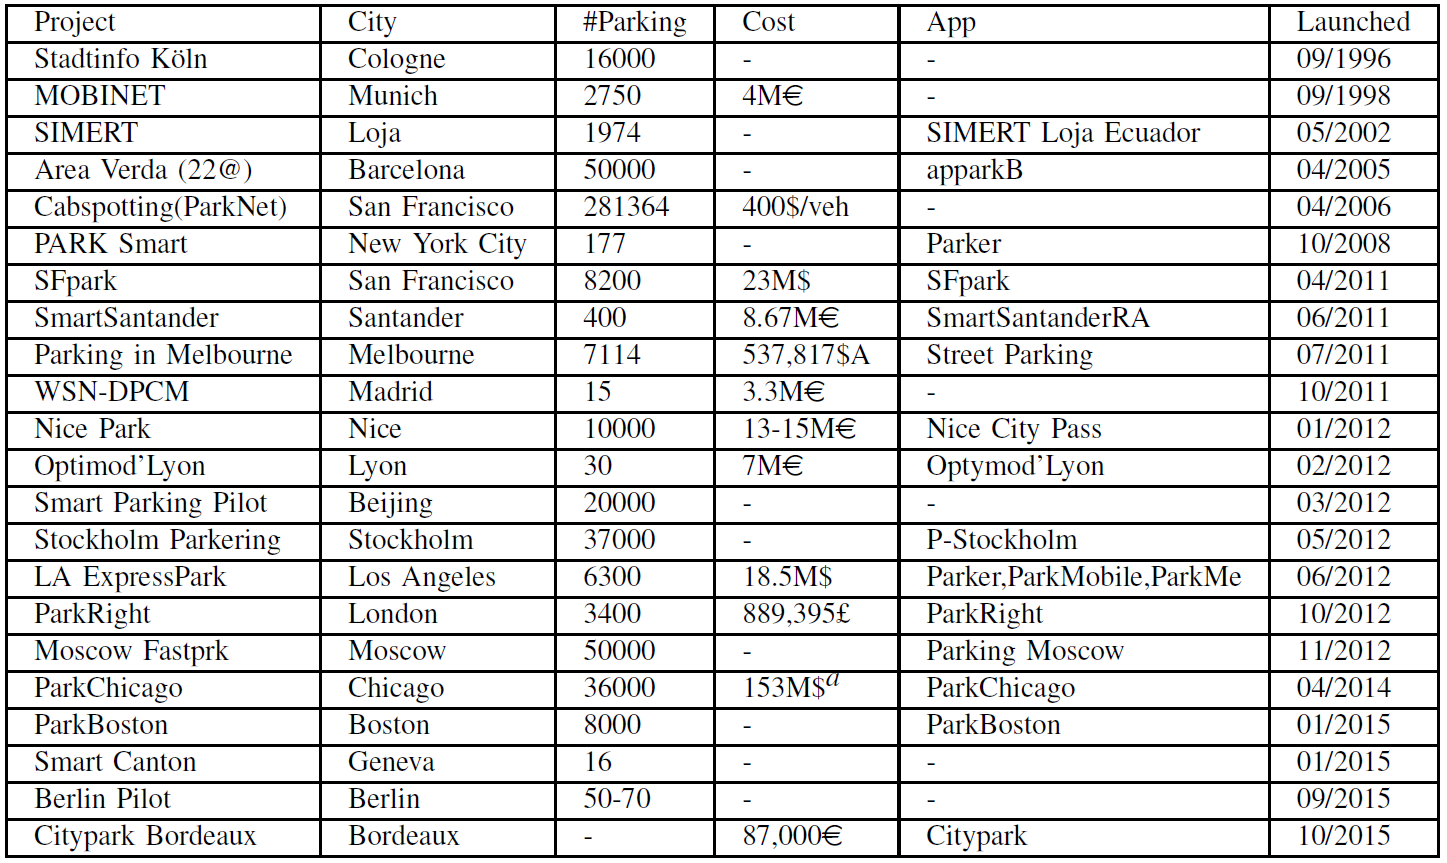
\includegraphics[width=0.8\textwidth]{graphics/related_work/smart_parking_projects.png}
%	\caption{Large-scale smart parking projects} %\cite{lin}
%	\label{fig:smart_parking_projects}
%\end{figure}

In the scientific literature there have been an increased number of publications on smart parking. We only touch upon some topics, such as parking reservation and resource allocation, our main focusing being occupancy prediction. We refer to a recent smart parking survey completed in 2017, that presents the developments in the field. The survey \cite{lin} is a follow-up to the main author's PhD thesis published in 2015 on the same topic \cite{lin2}. It presents the relevant developments on smart parking solutions since 2000. We shall use this survey to describe the research landscape for this topic. Afterwards, we will focus on parking prediction and we will go in depth on the relevant work done in that department. 

%As the research and development have been going in all directions, Lin et al. split the available results in \textit{information collection}, \textit{system deployment}, and \textit{service dissemination}.

%Under information collection, the authors include all techniques to acquire parking information. Be it static or mobile, in the form of sensors or as parking meters, the infrastructure here is diverse. Most of the time, the deployed sensors are managed through a wireless network infrastructure. The sensors are present inside cars, such as taxis, which travel through the city and collect  roadside information on parking. The piece of information transmitted is an occupancy change bit: either the car has left or arrived at a parking space. A number of types of sensors are usually being used in the process: infrared sensors, ultrasonic sensors, accelerators, optical sensors, inductive loops, piezoelectric sensors, cameras, acoustic sensors. Most of the time, the captured data requires post-processing in the form of image or audio recognition before arriving at the target occupancy information. Some of the captured information also raises privacy issues, at it contains sensitive data about the car and driver. Smartphones provide the means to collect data and can have a great impact through crowdsourcing, if the users are given incentives to enable the respective smartphone functions. On the other hand, there are systems where the driver initiates the data transmission. By using a mobile application, the driver may choose to report that he or she just left a parking space, respectively has arrived at a parking space. 

%In the system deployment section, the survey refers to the varieties of parking systems, looks into how well they scale, and touches upon their data analysis side. The parking systems software is the interface between the data sources and the users. Software systems are often in the form reservation systems, typically run by municipalities. Other systems also may provide guiding assistance in arriving at the desired parking space. Their vacancy prediction component informs the drivers about the availability of parking spaces at the destination. In this way, they contribute to the decision of the driver, of whether to take the car to the destination or not. Prediction systems recommend parking locations that have at least one parking space free.

%Under data dissemination, the authors of the survey address the ways in which parking data is exchanged between drivers. This scenario often occurs in decentralized parking systems, when the drivers find out about free parking spaces in an area where other cars drove by. Dynamic pricing is often used to control parking occupancy: parking prices are raised in areas that are almost fully occupied, whereas areas with low parking rates get assigned a lower price. A more advanced version adjusts the prices when enough demands received by the parking system would point to a future parking overload in the respective area. These approaches take into account parking competition: multiple drivers are looking to park in the same parking location.

%In order to view the related work comparatively, we have gathered the benchmark data from the relevant literature into \Cref{tab:related_work1}, which shows an overview of the systems presented in the papers, alongside the data sources used. Further specified are whether the system is dedicated to on- or off-street parking, and the location where it was evaluated.

%\begin{table}[!ht]
%	%\setlength\extrarowheight{5pt}
%	%\resizebox{\textwidth}{!}{%
%	%\centering
%	\tbl{Overview of all the systems introduced in individual articles}	
%	{\begin{tabular}{ | c | c | c | c | c | c |}
%			\hline
%			\textbf{Paper} & \textbf{Year} & \textbf{System} & \textbf{Data Sources} & \textbf{On/Off -Street} & \textbf{Location} \\ %\hline
%			
%			Caliskan \cite{caliskan} & 2007 & VANET & vehicle sensors & off-street & %\begin{tabular}{@{}c@{}}Brunswick,\\Germany\end{tabular}  \\ \hline
%			
%			Klappenecker \cite{klappenecker} & 2010 & VANET & vehicle sensors & off-street & - \\ \hline
%			
%			Wu \cite{wu} & 2014 & parking guidance & municipality & off-street & Taipei City \\ \hline
%			
%			Tiedemann \cite{tiedemann} & 2015 & parking prediction & sensors & on-street & Berlin \\ \hline
%			
%			Rajabioun \cite{rajabioun2013} & 2013 & parking guidance & \begin{tabular}{@{}c@{}} on-site sensors:\\ infrared, \\ %image-processing cameras,\\ inductor loops\end{tabular} & both & \begin{tabular}{@{}c@{}} Los Angeles,\\San Francisco\end{tabular} \\ %\hline
			
%			Rajabioun \cite{rajabioun2015} & 2015 & parking guidance & \begin{tabular}{@{}c@{}} sensors\\(cf. SF\textit{park} %\cite{sfpark})\end{tabular} & both & \begin{tabular}{@{}c@{}} Los Angeles,\\San Francisco\end{tabular} \\ \hline
			
%			Vlahogianni \cite{vlahogianni} & 2014 & routing system & \begin{tabular}{@{}c@{}} IoT nodes:\\ car presence \end{tabular}& on-street & Santander \\ \hline
			
%			Z. Chen \cite{zchen} & 2013 & \begin{tabular}{@{}c@{}}Location-based service\\ for parking finding\end{tabular} & manual collection & parking lots & Perth, Australia \\ \hline
			
%			Xu \cite{xu} & 2013 & parking prediction & mobile phone & on-street & San Francisco \\ \hline
			
%			X. Chen \cite{xchen} & 2014 & parking prediction & SF\textit{park} sensors & on-street & San Francisco \\ \hline
			
%			H\"ossinger \cite{hoessinger} & 2014 & parking prediction & \begin{tabular}{@{}c@{}}parking tickets\\ manual counts\\ traffic flow\end{tabular}& on-street & Vienna \\ \hline
			
%			Caicedo \cite{caicedo} & 2012 & parking reservation & in-cars sensors & both & Barcelona \\ \hline
			
%			Nandugudi \cite{nandugudi} &  2014 & parking prediction & smarphone & surface lots & Buffalo \\ \hline
			
%			Szczurek \cite{szczurek} & 2010 & VANET & GPS in car & both & - \\ \hline
			
%			Ji \cite{ji} & 2014 & parking guidance & - & off-street & Newcastle \\ \hline
			
%			Koster \cite{koster} & 2014 & parking recommender & smartphone & both & New York \\ \hline
			
%			Kotb \cite{kotb} & 2016 & parking reservation & occupancy sensors & - & - \\ \hline
			
%			Pullola \cite{pullola} & 2007 & parking prediction & GPS in car & on-street & Ottawa \\ \hline
			
%			Richter \cite{richter} & 2014 & - & SF\textit{park} sensors \cite{sfpark} & on-street & San Francisco \\ \hline
			
%			Shin \cite{shin} & 2014 & - & \begin{tabular}{@{}c@{}}sensors \\parking facilities \\cruising cars\end{tabular} & both & Luxembourg \\ \hline
			
%			Zheng \cite{zheng} & 2015 & - & parking sensors & on-street & \begin{tabular}{@{}c@{}} San Francisco \\Melbourne \end{tabular} \\ \hline
%	\end{tabular}}%
	%	}
%	\label{tab:related_work1}
%\end{table}

%\subsection{Vacancy Prediction Systems}
%\label{sec:relwork_vacancy_prediction}

%On the topic of prediction, there are a number of papers that approach the problem. The circumstances differ in each case, so that it is worth mentioning the papers individually first. Afterwards we will attempt to compare these approaches by extracting the most relevant aspects, e.g. method, type of data, features, error, deployment location, etc., in a table. 

%As in \Cref{sec:relwork_smart_parking}, all relevant work found on the topic are listed in Tables \Cref{tab:related_work2} and \Cref{tab:related_work3}. The key data shown emphasizes the prediction character of the papers by highlighting their general approach, features, methods, and evaluation.

%\begin{table}[!ht]
%	%\setlength\extrarowheight{5pt}
%	%\resizebox{\textwidth}{!}{%
%		\centering
%		\tbl{Overview of all the prediction methods used in related work}	
%		{\begin{tabular}{ | c | c | c | c | c |}
%			\hline
%			\textbf{Paper} & \textbf{Approach} & \textbf{Features} & \textbf{Methods} & \textbf{Evaluation}\\ \hline
			
%			Caliskan \cite{caliskan} & parking prediction & \begin{tabular}{@{}c@{}}age of parking info, \\arrival time, \\total capacity, \\occupancy, \\arrival rate, \\parking rate \end{tabular} & Markov chains & \begin{tabular}{@{}c@{}}probability density, \\ relative deviation\end{tabular} \\ \hline
			
%			Klappenecker \cite{klappenecker} & parking prediction & \begin{tabular}{@{}c@{}}total capacity, \\occupancy, \\arrival rate, \\parking rate \end{tabular} & Markov chains & - \\ \hline 
			
%			Wu \cite{wu} & parking recommendation & occupancy & probabilistic & \begin{tabular}{@{}c@{}}historical mean, \\moving average \end{tabular} \\ \hline
			
%			Tiedemann \cite{tiedemann} & parking prediction & occupancy & \begin{tabular}{@{}c@{}}data threads\end{tabular}& - \\ \hline
			
%			Rajabioun \cite{rajabioun2013} & parking prediction & \begin{tabular}{@{}c@{}}pricing, \\events, \\location, \\total capacity, \\occupancy rate, \\leaving rate \end{tabular} & probabilistic & mean error \\ \hline
			
%			Rajabioun \cite{rajabioun2015} & parking prediction & \begin{tabular}{@{}c@{}}occupancy, \\total capacity \end{tabular} & \begin{tabular}{@{}c@{}}multivariate-\\autoregressive \\model \end{tabular} & \begin{tabular}{@{}c@{}}orthogonality error \\differential covariance \\mean absolute \\-percentage error \end{tabular} \\ \hline
			
%			Vlahogianni \cite{vlahogianni} & parking prediction & \begin{tabular}{@{}c@{}}free space duration, \\occupancy, \\traffic volume, \\type of day, \\time period \end{tabular} & \begin{tabular}{@{}c@{}}genetically optimzed, \\multilayer perceptron\end{tabular} & Weibull distribution \\ \hline
			
%			Z. Chen \cite{zchen} & parking prediction & parking times & fuzzy logic & \begin{tabular}{@{}c@{}}occupancy error \\shortest travel time\end{tabular} \\ \hline
			
%			Xu \cite{xu} & real-time estimation & parking times & \begin{tabular}{@{}c@{}}Kalman \\adaptive linear memory filter\end{tabular} & RMSE \\ \hline
			
%			X. Chen \cite{xchen} & parking prediction & \begin{tabular}{@{}c@{}}events, \\distance, \\price \end{tabular} & \begin{tabular}{@{}c@{}}ARIMA, \\ linear regression, \\SVM, \\feed forward neural network \end{tabular} & MAPE \\ \hline
			
%			H\"ossinger \cite{hoessinger} & parking prediction & occupancy rate & \begin{tabular}{@{}c@{}}linear regression, \\average \end{tabular} & RMSE \\ \hline
			
%			Caicedo \cite{caicedo} & parking prediction & \begin{tabular}{@{}c@{}}capacity, \\price, \\occupancy \end{tabular} & probabilistic models & average error \\ \hline
			
%			Nandugudi \cite{nandugudi} & parking prediction & parking times & probabilistic model & absolute error \\ \hline
			
%			Szczurek \cite{szczurek} & parking prediction & parking times & \begin{tabular}{@{}c@{}}MALENA algorithm, \\Naive Bayes \end{tabular} & \begin{tabular}{@{}c@{}}average discovery \\time improvement\end{tabular} \\ \hline
			
%			Ji \cite{ji} & parking prediction & parking times & wavelet neural network & MSE \\ \hline
			
%			Koster \cite{koster} & parking recommendation & parking times & Markov chains & Pearson coefficient \\ \hline
			
%			Kotb \cite{kotb} & - & - & \begin{tabular}{@{}c@{}}Mixed-integer \\Linear Programming\end{tabular} & - \\ \hline
			
%			Pullola \cite{pullola} & parking prediction & parking times & Poisson process & absolute error \\ \hline
			
%			Richter \cite{richter} & parking prediction & see SF\textit{park} \cite{sfpark_evaluation} & time series model & absolute error \\ \hline
			
%		\end{tabular}}%
%	%}
%	\label{tab:related_work2}
%\end{table}


%\begin{table}
%	\tbl{Continuation of \Cref{tab:related_work2}}
%	{\begin{tabular}{| c | c | c | c | c |}
%		\hline
%		\textbf{Paper} & \textbf{Approach} & \textbf{Features} & \textbf{Methods} & \textbf{Evaluation}\\ \hline
		
%		Shin \cite{shin} & parking prediction & \begin{tabular}{@{}c@{}}driving duration, \\distance, \\walking distance, \\parking cost, \\traffic \end{tabular} & heuristic & \begin{tabular}{@{}c@{}}average driving duration, \\average walking distance, \\parking fail rate, \\parking utilization rate, \\average occupancy \end{tabular} \\ \hline
	
%		Zheng \cite{zheng} & parking prediction & parking occupancy & \begin{tabular}{@{}c@{}}regression trees, \\neural network, \\SVM \end{tabular} & MSE, $R^2$ \\ \hline
%	\end{tabular}}
%	\label{tab:related_work3}
%\end{table}
	
Xu et al. \cite{xu} makes real-time parking availability estimations based on a system that aggregates the data coming from mobile phones. The system uses algorithms based on statistical weighted schemes and Kalman filters. Additionally, the authors create parking availability profiles based on historical data and using statistical algorithms.

Chen et al. \cite{zchen} develop an Android application that finds a parking location at park-and-ride facilities by calculating the probability of parking availability and taking in consideration the shortest travel time. The authors employ fuzzy logic to model the uncertainty of parking availability. The fuzzy membership function was chosen to be linear. The authors proposed multiple criteria in finding the best parking location, such as train frequency, service quality, parking-and-ride price, which should be considered in further investigations. The use case and parking data were set in Perth, Australia.

Vlahogianni et al. \cite{vlahogianni} define prediction measures to find out the duration of free parking spaces. Additionally, they calculate 1-hour parking availability forecasts. The authors use neural networks for time-series in the form of a multilayer perceptrons to accurately predict occupancy up to one hour ahead. Their findings show a Weibull distribution for the duration of free parking spaces. The system developed was incorporated into the routing service of the city of Santander, Spain.

Rajabioun and Ioannou \cite{rajabioun2013} introduce an information system for parking guidance that enables communication between vehicles and the infrastructure. It proposes a prediction algorithm that forecasts the availability for parking locations based on real-time parking information. It takes into account parameters such as parking duration, arrival time, destination, pricing, walking distance, parking capacity, rates of vehicles occupying and leaving parking spots, time restrictions, parking rules, events that disrupt parking availability, etc. Their algorithm uses a probabilistic density distribution model. The parking data was collected both from on-street parking meters and off-street garages in Los Angeles and San Francisco, USA. In a following paper, Rajabioun and Ioannou \cite{rajabioun2015} propose a multivariate autoregressive model that considers the temporal and spatial correlations of parking availability when making predictions
%(cf. \Cref{fig:related_work_rajabioun})
. The authors hold that the model, which is integrated into a parking guidance and information system, recommends parking locations with high accuracy. 

%\begin{figure}[!ht]
%	\centering
%	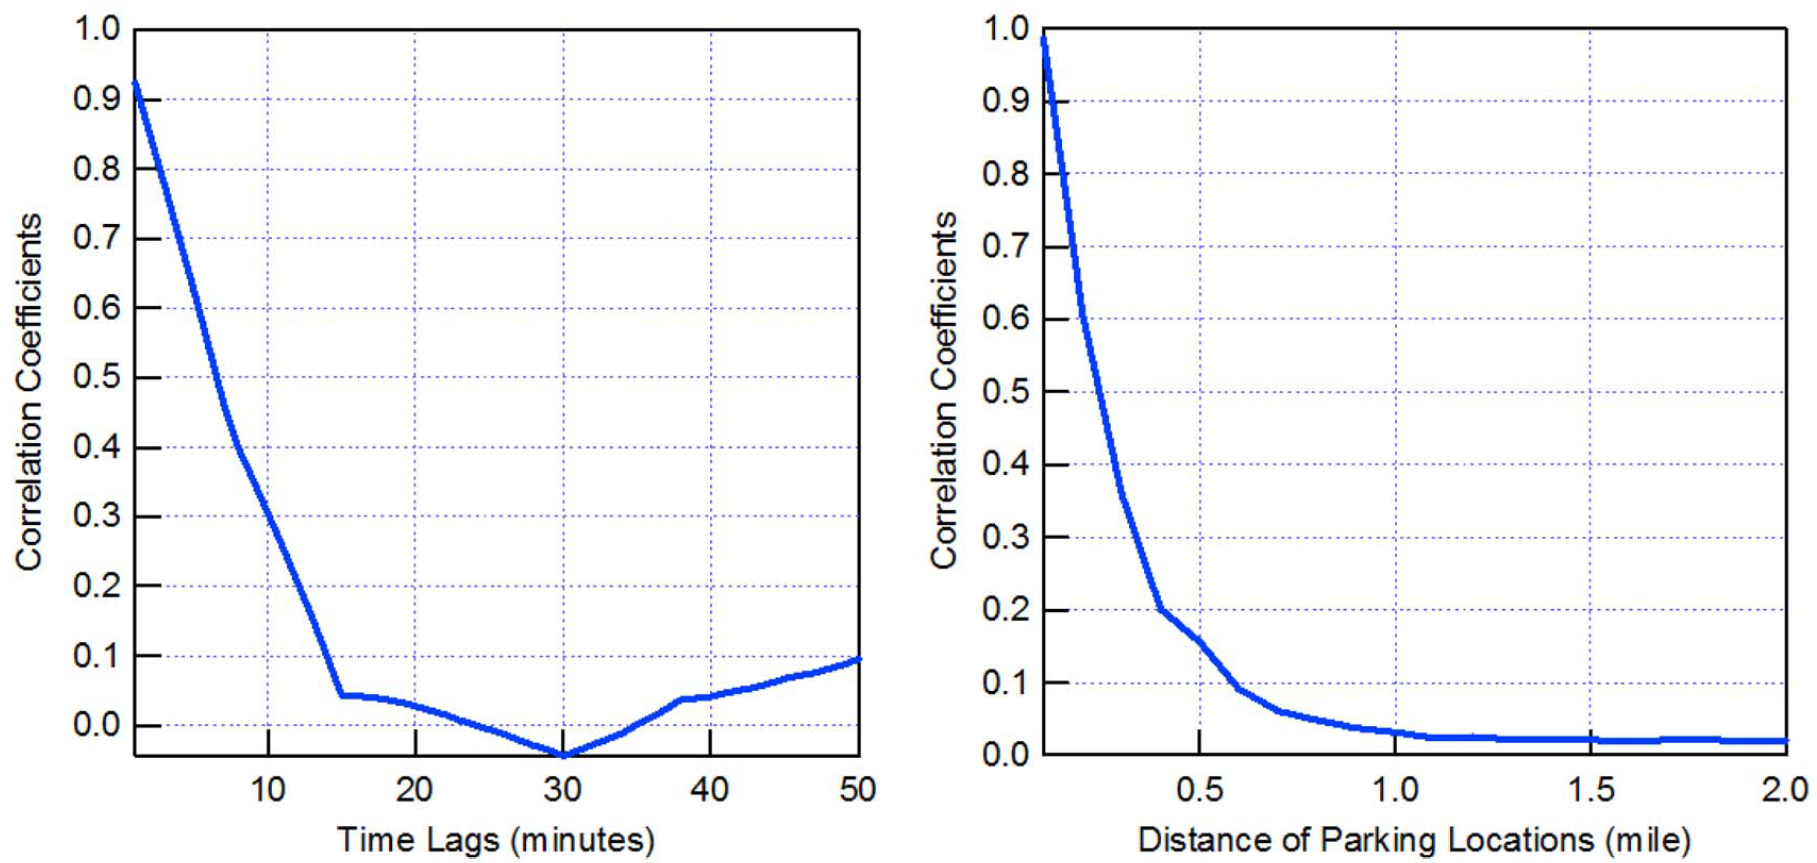
\includegraphics[width=0.8\textwidth]{graphics/related_work/rajabioun_1.png}
%	\caption{Left: Temporal correlation for parking occupancy Right: Spatial correlation for parking occupancy. Data collected from on-street locations in San Francisco} %\cite{rajabioun2015}
%	\label{fig:related_work_rajabioun}
%\end{figure}

Tiedemann et al. \cite{tiedemann} present the development of a prediction system that gives estimated occupancies for parking spaces. The occupancy data is collected online via roadside parking sensors and the prediction is realized using neural gas machine learning combined with data threads. The authors notice that some factors play a significant part in the predictions, such as holidays, weather and use the neural gas clustering to separate the data, before the data thread method is applied
%(cf. \Cref{fig:related_work_tiedemann})
. The system is developed by the DFKI Robotics Innovation Center, while the sensors are manufactured by Siemens AG and are installed in street lights. The pilot region for the project is Berlin, Germany.

%\begin{figure}[!ht]
%	\centering
%	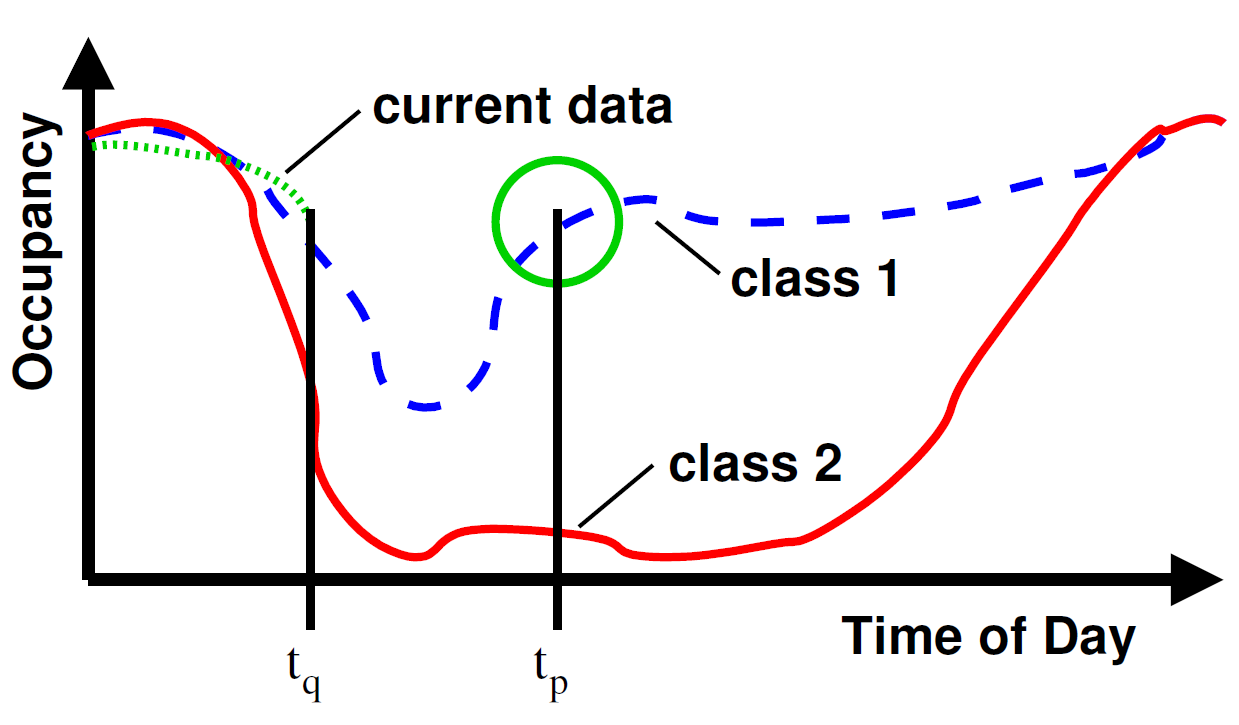
\includegraphics[width=0.8\textwidth]{graphics/related_work/tiedemann_1.png}
%	\caption{Visualization of data threads that are used for predicting occupancy. Class 1 (dashed blue curve) and Class 2 (solid red curve) are two learned time series. When the user queries for the occupancy prediction at $t_q$ for time $t_p$, the curve that is closest to the current data curve (dotted green) up to that point is chosen} %\cite{tiedemann}
%	\label{fig:related_work_tiedemann}
%\end{figure}

Wu et al. \cite{wu} present a information system that recommends parking options in the city, in order to reduce the vehicle emissions and decrease traffic. The system constructs an optimal parking sequence based on the forecasted parking availability. For the latter, probabilistic algorithms are used, i.e., shift prediction, thread estimation and probability estimation. The data and experimental results have been carried out in Taipei City in 2011.

Caliskan et al. \cite{caliskan} model the prediction of available parking spaces as a vehicular ad-hoc network (VANET). The network disseminates parking data in order to help with the estimation of future occupancy of parking lots. The pieces of disseminated data are timestamp, total capacity of parking lot, number of parking spaces that are currently occupied, the arrival rate, and the parking rate. The latter two are used in the modeling of continuous-time homogeneous Markov chains. The approach is otherwise based on queuing theory. The evaluation was carried out in Brunswick, Germany, where about 10000 vehicles were connected in the ad-hoc network. Klappenecker et al. \cite{klappenecker} builds on the result of Caliskan and uses an improved version of continuous-time Markov chains for predicting availability of parking spaces. Predictions are communicated between cars in an ad-hoc network. The approach simplifies the computations of transitional probabilities inside a Markov chain model. The system applies to parking lots that are connected to the ad-hoc network. These communicate the number of occupied spaces, capacity, arrival and parking rate. Also based on VANETs is Szczurek et al. \cite{szczurek} work, which propose a novel approach that combines machine learning with the information disseminated in ad-hoc vehicular networks. The building block of the system are parking reports, which are issued by vehicles leaving a parking space and comprise a report identifier, a location, and a timestamp. The parking reports are being learned by a model, which then indicates whether a parking is available for a specific vehicle. A conditional relevance is used to determine whether a particular report is useful for a specific vehicle. This is modeled using a Naive Bayes method. A parking availability report R is labeled relevant by vehicle V, if the parking space referenced in R is available when V reaches it. Upon evaluation of the methods, the authors reported an improvement in parking discovery times for vehicles.

PocketParker is a crowdsourcing system, proposed by Nandugudi et al. \cite{nandugudi}, that uses smartphone data to predict parking availability. The system is used for parking lots. It requires no input from the user, it notices automatically when a user starts to drive or stops, i.e., departure and arrival events
%(cf. \Cref{fig:related_work_nandugudi})
. Based on these two events, the system builds a probability distribution model that is used to answer queries about parking availability. PocketParker has proved robust to hidden parkers, i.e., parking vehicles that are not using the application. In the authors' simulation, it has reached 94\% rate for parking availability prediction with 105 users over 45 days.

%\begin{figure}[!ht]
%	\centering
%	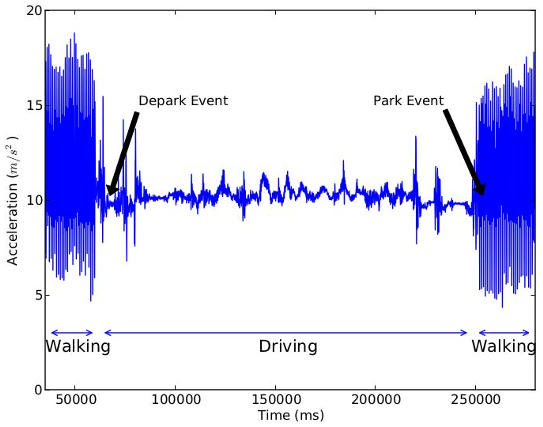
\includegraphics[width=0.8\textwidth]{graphics/related_work/nandugudi_1.png}
%	\caption{PocketParker detects a parking event using accelerometer data from the driver's smartphone } %\cite{nandugudi}
%	\label{fig:related_work_nandugudi}
%\end{figure}

Caicedo et al. \cite{caicedo} develop a methodology for predicting real-time parking space availability. The probabilistic algorithm consists of three subroutines: allocating simulated parking requests, estimating future departures, and forecasting parking availability. The forecast has been reported to improve as the system registers arrivals and departures. Further factors taken into account were duration of stay and capacity of every operating parking facility. The system was tested in Barcelona, Spain, with very satisfactory results.

H\"ossinger et al. \cite{hoessinger} present a simple real-time occupancy model based on various pieces of data collected in the city of Vienna, Austria. An average day curve model was built using the ticket data from mobile-phone parking, the counts of car parks, and the traffic flow volumes in the city.  The data was collected following agreements with the respective mobile phone companies, through surveys and by accessing a dedicated traffic website, respectively. The predictions are valid for short-time spans and applicable to the above mentioned city.

Chen \cite{xchen} tackles the parking problem by aggregating parking lots. The paper shows that the prediction  error of parking occupancy decreases by combining multiple parking lots. The trained models take into account factors such as day, time, event, distance, parking price, etc. The author tries out multiple models, such as ARIMA, linear regression, support vector regression and feed forward neural network. It turns out that the neural networks algorithm scores the best when the model is evaluated on the SF\textit{park} data \cite{sfpark_open_data}. Furthermore, the paper investigates the specifics of aggregated parking lots 
%(cf. \Cref{fig:related_work_xchen}) 
and finds certain artifacts in the occupancy graph when clustering the respective parking locations.

%\begin{figure}[!ht]
%	\centering
%	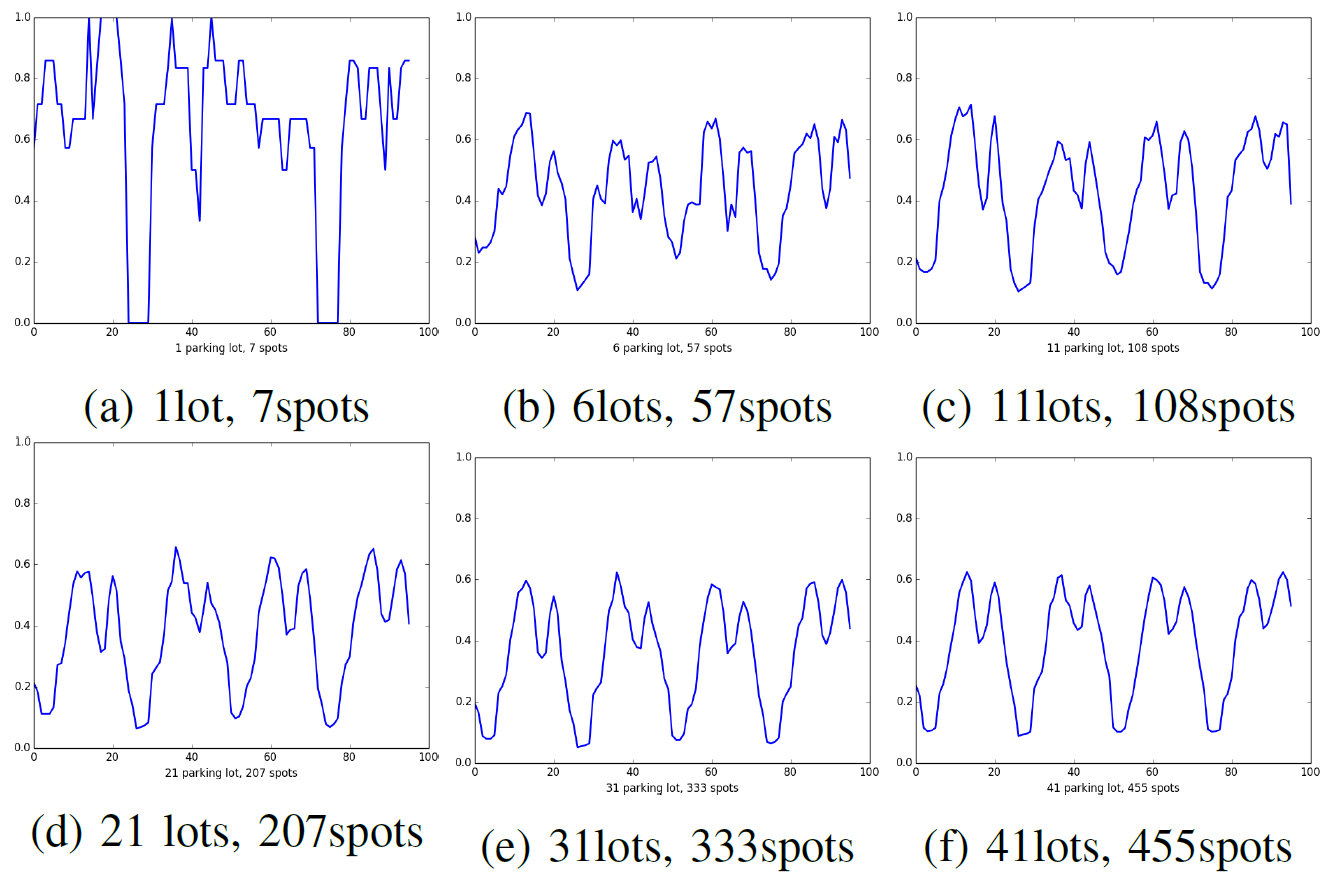
\includegraphics[width=0.8\textwidth]{graphics/related_work/xchen_1.png}
%	\caption{Increasing aggregation levels of parking lots. The more parking spaces are included, the smoother is the emerging pattern } %\cite{xchen}
%	\label{fig:related_work_xchen}
%\end{figure}

Richter et al. \cite{richter} address the parking prediction problem with the focus on model storage in vehicles. The authors train models of various granularity that would predict parking availability based on the information contained: a one-day model per road segment, a three-day model per road segment, and a seven-day model per road segment. Additionally, models based on regions and time intervals computed by clustering are tried out. Hierarchical clustering with complete linkage is employed. The models are evaluated on street data from the SF\textit{park} project \cite{sfpark_open_data}. The application of clustering before building the models shows a 99\% decrease of model storage space. The prediction success rate is at about 70\%.

With iParker, Kotb et al. \cite{kotb} propose a system that handles parking reservations. It achieves resource allocation so that drivers will pay less for parking, while parking managers receive more resource utilization and hence reach higher revenue. The system is based on mixed-linear programming (MILP). The system uses dynamic resource allocation and pricing models to achieve its goal. At its evaluation, it was reported to cut the cost for drivers by 28\%, achieving a 21\% increase in resource utilization, and it increased the total revenue for parking management by 16\%. Although this work only indirectly deals with parking occupancy, it makes use of it in a system that could include prediction models in the future.

%\begin{figure}[!ht]
%	\centering
%	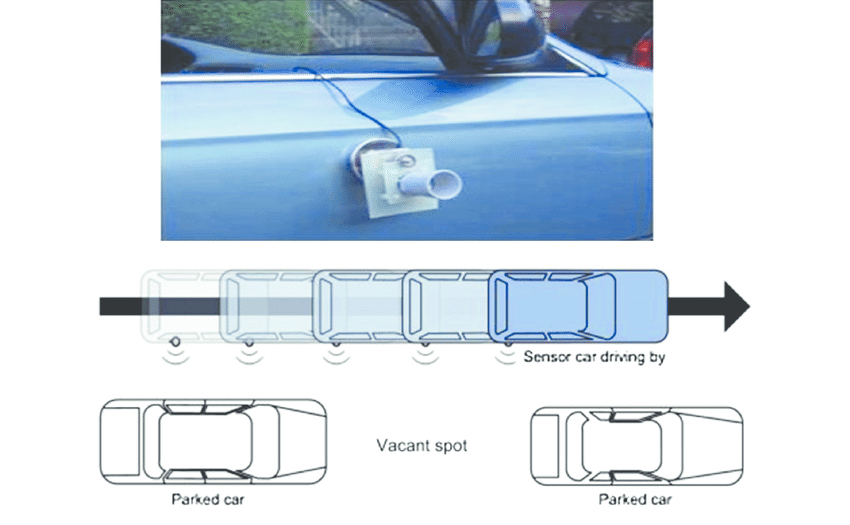
\includegraphics[width=0.8\textwidth]{graphics/related_work/mathur_1.png}
%	\caption{The ultrasonic sensor mounted sideways on cars in the ParkNet system } %\cite{mathur}
%	\label{fig:related_work_mathur}
%\end{figure}

ParkNet, developed by Mathur et al. \cite{mathur} is a system made up of vehicles that captures parking space information while driving. Every ParkNet vehicle is equipped with a GPS receiver and an ultrasonic sensor facing sideways
%(cf. \Cref{fig:related_work_mathur})
. The latter determines whether it passes by parking spaces and whether they are occupied. The data is sent to a central server that aggregates it, in order to build parking space occupancy maps in real-time. The information is queried by clients that search for a free parking space. The system was evaluated in Highland Park, New Jersey and San Francisco on 500 miles road-side parking data and yield 95\% accurate parking maps and 90\% parking occupancy accuracy. The authors show that the system can further be improved if the sensors are fitted into taxicabs or city buses.

Ji et al. \cite{ji} presents a forecasting method based on wavelet neural networks. These are feed-forward neural networks that have continuous wavelet function as activation function for the hidden layers. The system was tested in Newcastle upon Tyne, England and evaluation was performed using real-time data of up to 1 day in advance.

Koster et al. \cite{koster} propose a smartphone-based solution that recognizes when drivers arrive or leave parking spaces. A ``Bayesian approach'' and Hidden Markov Models (HMM) are used to model the parking spaces and respond to user queries for the next parking space. The HMM are based on gathered historical data. As answer to the user query is a parking space nearby and the probability of it being free at the respective time. The authors emphasize the non-intrusive nature of the solution, where drivers only have to minimally interact with their phones to get a recommended free parking space.

Pullola et al. \cite{pullola} propose a solution to determine the availability of parking lots by modeling the occupancy as a non-homogeneous Poisson process. Past occupancy information of the parking lots is stored and leveraged. The data and the computation are made inside the GPS system of the vehicle, in order not to depend on the quality of the transmitted signal. 

Zheng et al. \cite{zheng} investigates the results of a proposed prediction mechanism on the parking data collected in San Francisco and Melbourne. The three algorithms proposed employ regression trees, support vector regression and neural networks. The feature sets included the historical occupancies alongside the time and day of the week.

Shin and Jun \cite{shin} propose an algorithm for smart parking that assigns cars to parking facilities in the city. The criteria based on which the assigning is realized includes driving distance to the parking facility, walking distance from the parking facility to the destination, parking cost, and traffic congestion. The real-time data is collected from parking facilities and from sensors that are integrated in cruising cars. The data is transferred from the central server, where it is managed through a wired/wireless telecommunication network. The authors test their approach in Luxembourg City. The results of the simulations showed improved figures for average driving duration, average walking distance, parking failing rate, parking utilization rate, average standard deviation on the number of guided cars to each parking facility, average occupancy ratio of parking facility, and for the parking facility occupancy rate.  

While all the presented approaches tackle the problem of improving the parking situation in cities with different ideas and implementations, they fundamentally differ from our work. 
Some approaches match with our idea of adding additional information about the current circumstances in a city or by building models for smaller areas.
However, none of the approaches focuses on building a solution that can be ported to other cities. 
As opposed to this, our presented approach uses a public pre-defined ontology and data in RDF format as input in order to calculate the prediction models and similarity measures. 
Further, none of the presented approaches aims at training prediction models for small areas where data are available and transfer those models to other areas where no data is available. Our approach aims exactly at this goal for enabling a more accurate prediction in districts or streets where no parking data are available. 

\section{Selected Data Source}
To implement and evaluate our idea, we use the data from the SF\textit{park} project. This project was realized by the San Francisco Municipal Transportation Agency (SFMTA), the city agency that manages the city's transportation, which includes on-street parking~\cite{sfpark} \cite{sfpark_evaluation}. The SFMTA establishes parking rates for on-street parking meters. Before the project started, parking rates were the same all day, every day, independent of the parking demand. By implementing a demand responsive pricing scheme, parking availability improved dramatically. 
%The facts listed in \Cref{tab:sfpark_results} show the improvements on parking after the project completed.

%\begin{table*}
%	\centering
%	\begin{tabular}{c}
%		\toprule
%		\begin{minipage}{0.7\textwidth}
%			\begin{itemize}
%            %	\itemsep 0.5em
%				\item the amount of time parking areas were too full decreased by 16\%
%				\item the amount of time to find a parking space decreased by 43\%
%				\item parking citations decreased by 23\%
%				\item traffic volume decreased by 8\% in the pilot areas
%				\item the average hourly rate was overall decreased by 11 cents, from \$2.69 to \$2.58
%				\item double-parking decreased by 22\%
%				\item there was a 30\% drop of greenhouse gas emissions per day (originally 7 cubic meters tons)
%				\item there was an increase in \$1.9M annual revenue, although raising revenue was not a goal of the project
%			\end{itemize}
%		\end{minipage}
%		\\ \bottomrule
%	\end{tabular}
%	\caption{The main results from the SF\textit{park} project}
%	\label{tab:sfpark_results}
%\end{table*}

In conducting the project, nine pilot areas were chosen for monitoring. Out of these areas, seven were selected to have new pricing policies, while two were control areas. The number of metered spaces used was 6000, which amounts for 25\% of the city's total. The meters allow rates to be deployed remotely and they transmit data to a central server through a wireless connection.

The data was collected using parking sensors. These provided the central server with the information needed to calculate the demand-responsive parking rates and provided real-time parking availability information. A parking sensor is a magnetometer that detects changes in the earth's electromagnetic field. A total of 11700 sensors were deployed, resulting in 8000 spaces that were equipped with one or two sensors. The sensors delivered valid data from April, 2011 to December, 2013. The sensors can suffer from environmental noise, such as electromagnetic interference, early battery degradation or street construction. 

SF\textit{park} made available real-time information on parking rates and parking occupancy through a smart phone application. The SF\textit{park} project and its success played an important role when choosing to base our project on it.

\section{Concept}
For implementing our approach, we extract parking data from SF\textit{park}. In addition, we collect city data from various sources (cf. \Cref{sec:citydata}). To ensure that our approach will be compatible with data available in other cities, we annotate our data using ontologies from the CityPulse project~\cite{city_pulse} and store them in RDF format. Afterwards, we merge the data sets and perform a clustering process. Next, we define the parking profile by introducing two similarity functions: \textit{cosine similarity} and \textit{earth mover's distance}.
Finally, we explain the machine learning training process and define the estimations for clusters without parking data.

%\begin{figure}
%	\centering
%	\fbox{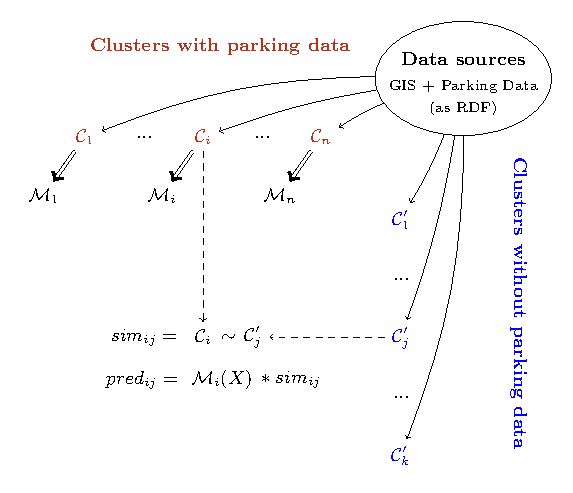
\includegraphics[width=0.45\textwidth]{graphics/concept_overview}}
%	\caption{Concept Visualization}
%	\label{realization:concept_overview}
%\end{figure}

\subsection{Parking Data}
We consider the following types of data as parking data: \textit{parking occupancy} contains information on the availability of parking spaces; \textit{traffic data} contains information regarding the city traffic, which is relevant for parking; \textit{weather data} contains weather information for the same area as for the parking problem; \textit{event data} contains event information which may have an impact on parking; \textit{parking revenue data} contains economic information on parking, whose relevance may influence parking prediction. \textit{fuel price data} contains prices of fuel in the region for which we build the models.
Each piece of data is geographically referenced by a \textit{location unit}, e.g., street block, district or city. 
An overview of the different properties available in the data set are shown in \Cref{tab:sfpark_data}.

\begin{table}
	\tbl{An overview of the properties available in the data used from the SFpark project}
	{\begin{tabular}{lp{4cm}lp{4cm}}	
		\toprule
		Parking Occupancy & & Traffic & \\
		%\midrule
		\colrule
		date and time & Recorded usually at full hours or in periodic time intervals & date and time & recorded usually at full hours or in periodic time intervals \\
		parking capacity & The total number of parking spaces at the given location & traffic value & typically expressed as average traffic road occupancy, average vehicle count, median speed, or average speed of the traveling cars \\
		parking price & The price of a ticket at the certain location and the given time in a given currency & & \\
		parking occupancy & Expressed either as rate (subunitary fraction or percent) or in absolute numbers & & \\
		%\midrule
		\colrule
		Events & & Weather & \\
		%\midrule
		\colrule
		event name class & the name of the event and its class (road closure, rise of parking demand) & temperature & may be current temperatures or maximum and minimum values per day \\
		& & 	precipitation & expressing the quantity of rain or snow for the corresponding time interval \\
		%\midrule
		\colrule
		Fuel Price & & Parking revenue & \\
		%\midrule	 
		\colrule
		type of fuel & gasoline, diesel, etc. & payment type & the way the driver opted to pay for parking, e.g., cash, credit card, etc. \\
		
		price per unit & provided as the price per liter or per gallon. & payed amount & the amount in US dollars, Euro or other currency\\
		
		%\bottomrule
		\botrule
	\end{tabular}}
	\begin{tabnote}
		Each of these data types also has the location unit id, as well as the date and time (interval) when it occurred or was measured. 
		In some cases, the location is a somewhat larger or smaller area as the unit. The time information is provided in different granularities (e.g., per minute, per hour, per day, etc. )
	\end{tabnote}
	\label{tab:sfpark_data}
\end{table}

\subsection{City Data}
\label{sec:citydata}
We established that city data reflects parking demand in a city area. We obtain it by collecting public amenity information as provided by OpenSteetMap\footnote{\url{https://www.openstreetmap.org} The maps used in this article are \textcopyright OpenStreetMap contributors}. The OSM data is available as shapefiles containing geometries such as points, polylines and polygons. We extract the \textit{points of interest} (POIs). A POI contains an \textit{amenity} attribute indicating the public service located at this position as it was annotated by the OSM users (cf. \Cref{fig:pois}).

\begin{figure}[!ht]
	\centering
	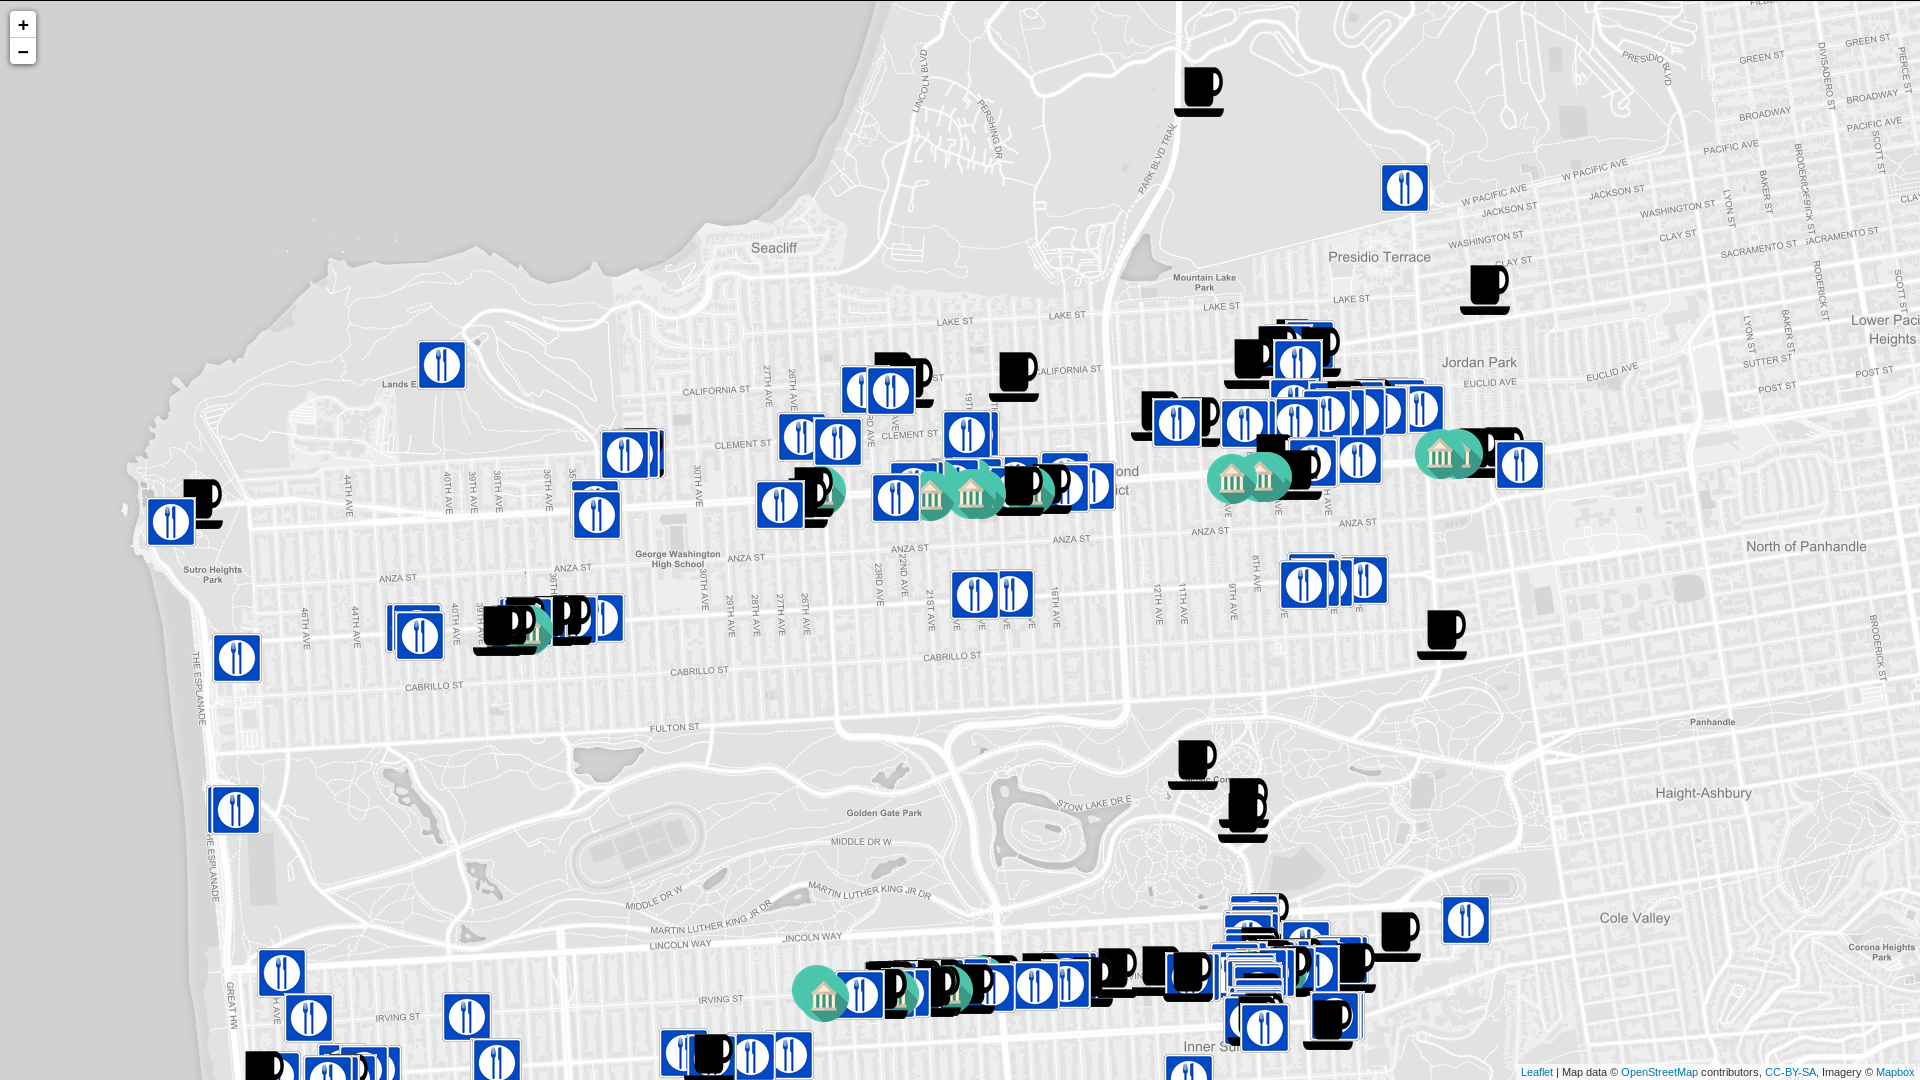
\includegraphics[width=0.8\textwidth]{graphics/cafes_restaurants_banks_larger.png}
	\caption{A map indicating public amenities (cafes, restaurants, banks) found at points of interest in OSM.}
	\label{fig:pois}
\end{figure}

The amenity information accounts for the times of parking (i.e., morning, day, night, etc.) and, up to some degree, for the duration of parking. An example of a service indicating this is Google Maps.
It displays typical \textit{visiting duration} or \textit{time spent} values and popularity of the place for specific points in time. The average values are based on the users' smart phone GPS sensors (cf. \Cref{fig:visit_duration}). To obtain the duration values, we manually extract information from Google Maps. The duration information is aggregated by Google using a crowdsourcing approach. 

\begin{figure}[!ht]
	\centering
	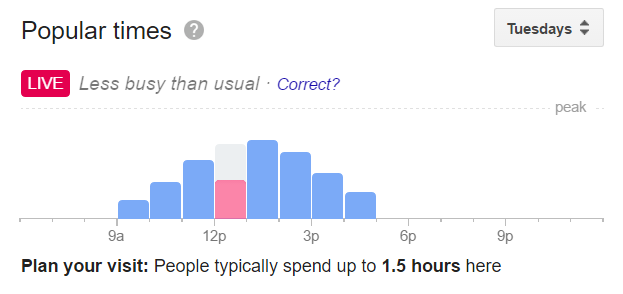
\includegraphics[width=0.8\textwidth]{graphics/google_visit_duration.png}
	\caption{An example of \textit{visiting duration} information found on Google Maps.}
	\label{fig:visit_duration}
\end{figure}

\subsection{RDF Annotation}
We emphasized that our approach should be relevant for any city that wants to solve its parking problem. Thus, all input data used in the present approach is in RDF format, in order to establish a common format that can be used for other cases.
Since the actual parking and city data is only available as raw values, we need to annotate it as RDF in the first place.
The default process involves the extraction of data, which is afterwards available for further processing. To annotate the city and parking data, we use Apache Jena. As underlying ontologies, we reuse those created as part of the CityPulse project~\cite{city_pulse}. Afterwards, we can easily extract the data in a well-defined format using SPARQL queries. 

\subsection{Merging City and Park Data}
In order to combine the parking and city data, both sets of data require a common location unit. 
The parking location units are provided together alongside the various types of parking data. 
The city data, on the other hand, references POI geometries, which are points expressed in a particular reference system, which differs from the one of the parking locations.
Therefore, after establishing the coordinate systems of both geometries, we define a \textit{merge distance} that matches a parking space to a public amenity. 

The merge distance can be intuitively understood as the radius around a public amenity. It is defined to represent the parking area that is relevant for a particular public amenity, or, more straightforward, the walking distance from the parked car to, e.g., the restaurant, the office, the bank, etc. Concrete instances of the merging distance can be found in \Cref{experimental_setup:merging_parking_city_data}.

\subsection{Clustering}
\label{concept:clustering}
In a realistic scenario, the available parking data does not cover the whole city surface. In fact, it is a fraction of it. Therefore, we first separate the area \textit{with} parking data from the area \textit{without} parking data. Based on this initial split, we perform clustering to further separate these regions into smaller areas. By splitting into city areas, we are making sure that smaller regions lead to more representative parking profiles and therefore parking estimations. 

As we want an exclusively location-based separation, we may employ K-Means, DBSCAN or OPTICS to cluster the city areas. The distance is calculated between (latitude, longitude)-pairs of location unit coordinates corresponding to one parking unit. There are two clustering processes executed, one for the city area \textit{with} parking data, another one for the city area \textit{without} parking data. The number of clusters chosen in each area is kept proportional to the number of total location units that each city area contains. Since having control over the number of clusters is the goal here, we choose to use K-Means, where we provide the number of expected clusters as input. More details on the concrete value of $k$ and an overview about the clusters can be found in \Cref{experimental_setup:clustering}.

\subsection{Similarity Functions}
\label{realization:similarity_functions}
To calculate the similarity of city areas, we use \textit{cosine similarity} and \textit{earth mover's distance}. For this, we use two representations of city areas: \textit{cluster vectors} and \textit{cluster Gaussians}. As data, we use the city data described in \Cref{sec:citydata}.

\subsubsection{Cosine Similarity}
\label{realization:vectors}
To form the cluster vectors, we first divide all amenities into categories $Cat_1, Cat_2, ..., Cat_n$.
The criteria for division will be their average \textit{visiting duration} duration.
For example, a short duration category of up to 30 minutes, a medium duration between 31 and 90 minutes and a large duration of above 90 minutes stay.
Each cluster gets represented by an $n$-dimensional vector, whose components correspond to the amenity categories.
The magnitude of component $i$ is equal to the number of amenities of category $Cat_i$ that can be found in that particular cluster.
Compare \Cref{fig:cluster_vector} for a general representation.

\begin{figure}[!ht]
	\centering
	\includestandalone[width=0.7\textwidth]{graphics/cluster_vector}
	\caption{An example of a cluster vector for three categories.}
	\label{fig:cluster_vector}
\end{figure}
%\label{realization:cosine_similarity}
The cosine similarity between two vectors is defined as the cosine of the angle between the two vectors:

\begin{equation}
cos(\theta)=\frac{A\cdot B}{{\lVert}A{\rVert}       
	_2{\lVert}B{\rVert}_2}=\frac{\sum_{i=1}^n{A_iB_i}}{\sqrt{\sum_{i=1}^n{A_i^2}}\sqrt{\sum_{i=1}^n{B_i^2}}}
\end{equation}
where $A_i$ and $B_i$ are the components of vector A, respective B. 

Unlike the earth mover's distance, the cosine similarity implementation uses the direct mathematical formula by plugging in the magnitudes of the respective vector components.

\subsubsection{Earth Mover's Distance}
\label{realization:gaussians}

A cluster Gaussian is a \textit{kernel density estimation} among amenity probability distributions.
In turn, an amenity probability distribution is represented as \textit{Gaussian kernel}.
To construct a cluster Gaussian, we first collect the average visiting duration and standard deviation for the individual amenities.
A cluster that contains one amenity $A$ is represented as a Gaussian curve, i.e., normal probability distribution.
The curve's center is at the average duration of the amenity $A$ and its standard deviation is the one of the amenity.
When $n$ amenities $A$ exist in the cluster, the representation will be an $A$ curve multiplied $n$ times.
Multiple amenities, each appearing multiple times, will result in a curve that is the linear combination of the individual representations of the amenities as normal distribution curves.
Compare \Cref{fig:gaussian} for a visualization of the summing process.

\begin{equation}
emd(\mathcal{C}_i) = \sum_{j=1}^{|amenities|} K_{ij} \times A_j
\end{equation}

$$\forall i \in \{1,..|clusters|\} \text{ and } \forall j \in \{1,..|amenities|\}$$

where $A_j$ is an amenity that appears $K_{ij}$ times in the cluster $\mathcal{C}_i$.

\begin{figure}[!ht]
	\centering
	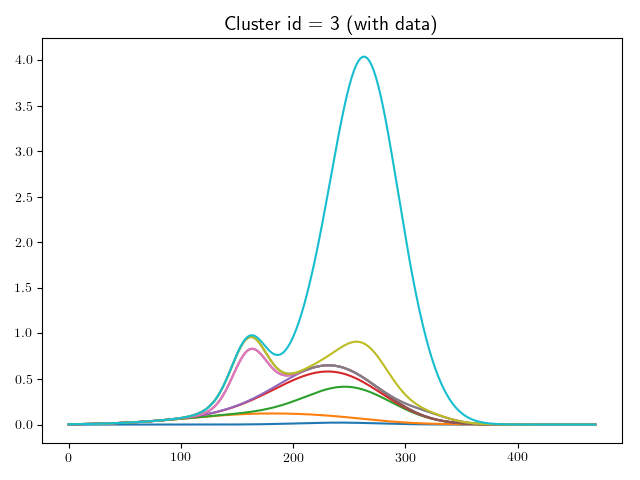
\includegraphics[width=0.8\textwidth]{graphics/emd_gaussian_addition3.png}
	\caption{The summing of Gaussians resulting in a cluster Gaussian.}
	\label{fig:gaussian}
\end{figure}

The earth mover's distance (emd) is a measure used in statistics that roughly expresses the difference between position and magnitude of two curves.
It is best explained by regarding the curves as the hull of earth piles.
For two separate earth piles, emd computes the minimum effort of rearranging a pile so that the shape of the other pile is obtained.
Moving P particles over a distance D is equal to the effort $P \times D$.
A prerequisite for this operation is that the two piles need to contain the same quantity of earth.

More rigorously, the earth mover's distance is better known in mathematics under the name Wasserstein Metric.
Given two normal distributions $\mu_1=\mathcal{N}(m_1,C_1)$ and $\mu_2=\mathcal{N}(m_2,C_2)$, where $m_1$ and $m_2 \in \mathbb{R}^{n}$ are their respective expected values and $C_1$ and $C_2 \in \mathbb{R}^{n\times n}$.
Then, the 2-Wasserstein distance between $\mu_1$ and $\mu_2$ is:

\begin{equation}
W_2(\mu_1,\mu_2)^2={\lVert}m_1-m_2{\rVert}^2_2+trace(C_1+C_2-2(C_2^{1/2}C_1C_2^{1/2})^{1/2})
\end{equation}

In practice, we will not apply the Wasserstein metric directly, but rather resort to some levels of discretization.
First off, a number of so-called bins is determined.
Each bin represents a unit on the $X$ axis, the same on which the visiting duration is expressed.
We will take a number of buckets equal to the maximum amenity mean and add $3\times$ the largest standard deviation to it, as it is known that within $3\times$ standard deviation on both sides of the mean over 99\% of the Gaussian sum is covered.
Moreover, an offset on the $X$-axis equal to $3\times$ the maximum standard deviation is used.
This way, we are sure the landscape of summed Gaussians will easily fit into the number of bins.

Notice that emd is applicable only when the sum under both Gaussian curves is equal.
Therefore, all cluster Gaussians will get normalized before emd is computed.

\subsection{Machine Learning Models}
\label{realization:machine_learning_models}
The prediction of parking occupancy is realized using machine learning.
We choose to explore this methodology, following the solid results machine learning models have delivered for the various smart parking settings investigated in \Cref{sec:relwork}. A machine learning model $\mathcal{M}$ will be trained for every cluster \textit{with} parking data.

The training data \textit{features} are composed of the parking data previously enumerated. We aggregate feature values around the location unit id, as on the cluster level this is irrelevant. The occupancy rate is set as the target variable. The model training and evaluation is performed in Python via the \textit{scikit-learn} library.

During the training phase, we evaluate different machine learning approaches ranging from simple decision trees over random forests to support vector machines and gradient boosting. In addition, we make use of grid search to determine the best model parameters for the current approach. As error metric, we use root mean square error and performed a ten-fold cross-validation. Furthermore, a model is evaluated on the other clusters with parking occupancy data.

\subsection{Parking Occupancy Estimations}
\label{realization:parking_occupancy_estimations}
Once all models $\mathcal{M}$ have been built for the clusters \textit{with} parking data, making estimations on parking occupancy in these areas is straightforward. However, we want to apply these models, on the clusters that are missing parking data. We derive the \textit{estimation interval} for cluster $\mathcal{C}_{wout}^j$ based on the model of cluster $\mathcal{C}_{with}^i$ as follows.

For cosine similarity:
\begin{equation}
E(\mathcal{C}_{with}^i,\mathcal{C}_{wout}^j) = [\mathcal{M}(\mathcal{C}_{with}^i) - (1 - sim_{ij}), \text{    } \mathcal{M}(\mathcal{C}_{with}^i) + (1 - sim_{ij})]
\end{equation}
$$\text{where } sim_{ij} = sim(\mathcal{C}_{with}^i,\mathcal{C}_{wout}^j) \in [0,1]$$

For earth mover's distance:
\begin{equation}
E(\mathcal{C}_{with}^i,\mathcal{C}_{wout}^j) = [\mathcal{M}(\mathcal{C}_{with}^i) - emd_{ij},   \text{    }\mathcal{M}(\mathcal{C}_{with}^i) + emd_{ij}]
\end{equation}
$$\text{where } emd_{ij} = emd(\mathcal{C}_{with}^i,\mathcal{C}_{wout}^j) \in [0,1]$$

$$\forall i \in \{0,...,|\mathcal{C}_{with}|-1\} \text{ and } \forall j \in \{0,...,|\mathcal{C}_{wout}|-1\}$$.

$X$ is a parking data record containing feature values.
The result is an \textit{estimation interval} that ``stretches'' the punctual estimation into an interval depending on the similarity value.
The lower the similarity value is, the larger the length of the resulting estimation interval will be.

Notice that $X$ should be valid for both $\mathcal{C}_{with}^i$ and $\mathcal{C}_{wout}^j$. The averaged values used for features related to the location unit id will be transferred as they are similar to those of the target cluster $\mathcal{C}_{wout}^j$.

Furthermore, we define an \textit{estimation intersection interval}, whose purpose is to narrow down the computed estimation interval.
An estimation intersection interval for the clusters $\mathcal{C}_{with}^i$ and $\mathcal{C}_{wout}^j$ is computed by intersecting the \textit{estimation intervals} that have a better similarity among the clusters with data $\mathcal{C}_{with}^{0}, ..., \mathcal{C}_{with}^{i-1}$ and the same cluster without data $\mathcal{C}_{wout}^j$.

\begin{equation}
EII(\mathcal{C}_{with}^i,\mathcal{C}_{wout}^j) = \bigcap_{k=0}^{i-1} EI(\mathcal{C}_{with}^k,\mathcal{C}_{wout}^j) \\
\end{equation}

where
\begin{equation}
sim(\mathcal{C}_{with}^k,\mathcal{C}_{wout}^j) < sim(\mathcal{C}_{with}^i,\mathcal{C}_{wout}^j), k \in \{0,..,i - 1\} \text{ for emd}\\
\end{equation}
\begin{equation}
sim(\mathcal{C}_{with}^k,\mathcal{C}_{wout}^j) > sim(\mathcal{C}_{with}^i,\mathcal{C}_{wout}^j), k \in \{0,..,i - 1\} \text{ for cosine} 
\end{equation}

$$\forall i \in \{0,...,|\mathcal{C}_{with}|-1\} \text{ and } \forall j \in \{0,...,|\mathcal{C}_{wout}|-1\}$$.

\section{Experimental Setup}
In the following, we describe the pre-evaluation setup, consisting of practical considerations on the following: parking- and city data, clustering, similarity functions, model training and testing, as well as data aggregation.
The first elements needed for evaluation are parking and city data. As parking data, we use those from the SF\textit{park} project and determine the data sets that are relevant for our purposes. As city data, we take OpenStreetMap data from San Francisco and obtain the available public amenity information. Google Places provides the visiting duration values for the amenities. Based on these data sets, we determine relevant values for the \textit{merge distance}. Since we cannot evaluate the performance of our approach using clusters \textit{without} data, we evaluated the performance on clusters for which occupancy data were available. 
Therefore, we first calculated the similarity score between every pair of clusters ($\mathcal{C}_{source}, \mathcal{C}_{target}$), after which the estimation errors were computed by applying the model of cluster $\mathcal{C}_{source}$ to $\mathcal{C}_{target}$, for all such pairs of clusters.

\subsection{SF\textit{park} parking data}
\label{experimental_setup:sfpark}
The SF\textit{park} data are visualized in Figure \ref{fig:before_clustering} using a Leaflet application built as part of this work.
The actual SF\textit{park} data has some peculiarities.
While the \textit{occupancy data} is provided with reference to \textit{blocks} as location units, all the other data sets use different location units.
For the traffic and events data sets, the location units are street names.
For parking revenue, they are districts.
In case of weather and fuel price, the location reference is valid for the whole city of San Francisco. 
Hence, there is a need to align the different data sets before they can be used together.

\begin{figure}[!ht]
	\centering
	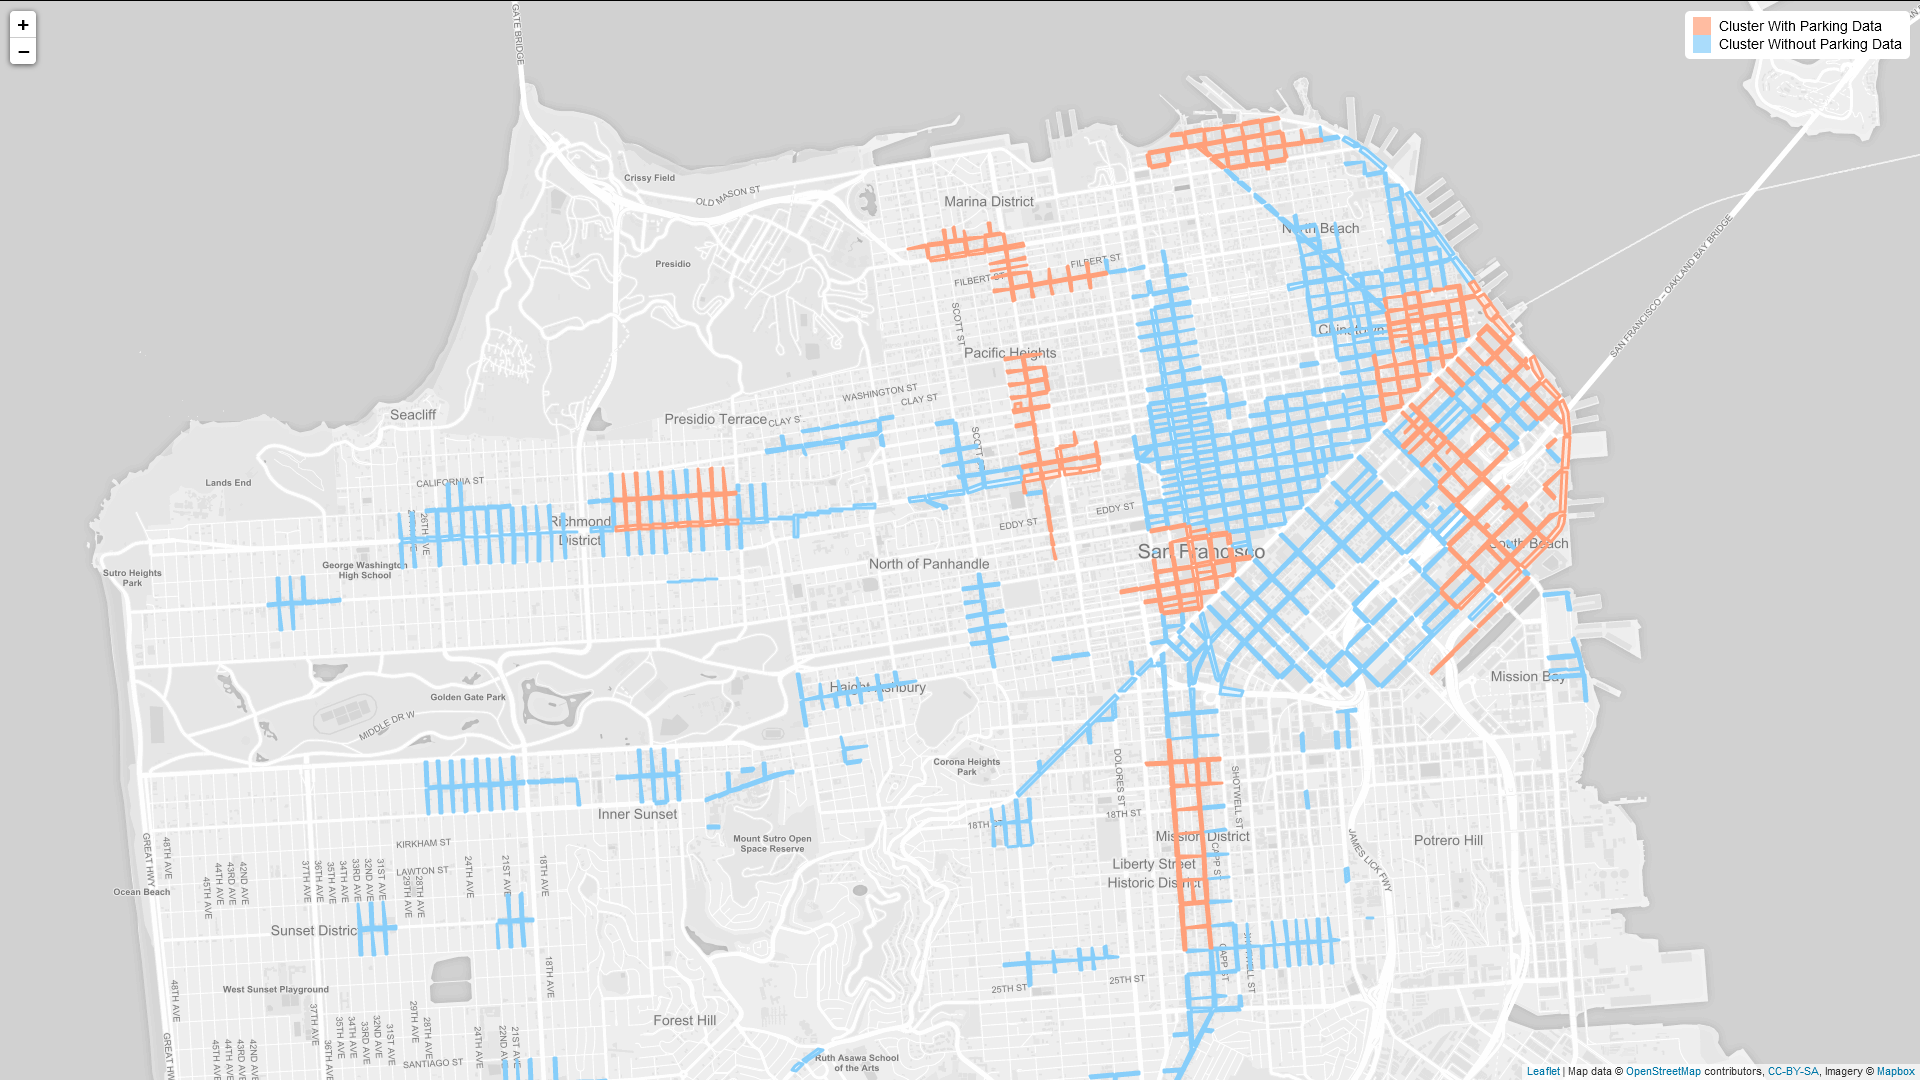
\includegraphics[width=0.8\textwidth]{graphics/initial_view_before_clusteringV7.png}
	\caption{The blocks accounted in SF\textit{park}. The light blue ones are blocks \textit{without} parking data, the light red ones are \textit{with} parking data.}
	\label{fig:before_clustering}
\end{figure}

\subsection{OpenStreetMap for San Francisco}
\label{experimental_setup:osm_for_sf}
Following the selection of SF\textit{park} data as parking data, the city data is found in the corresponding OpenStreetMap layer for San Francisco.
The types of the public amenities collected from the POIs are listed in \cref{tab:amenities_list}.

\begin{table}[!ht]
	%\scriptsize
	\tbl{List of all OSM amenities found in the SF\textit{park} blocks.}
	{\begin{tabular}{ | l l l l l | }
		\hline
		arts\_centre & dojo & marketplace & shelter & conference\_centre \\
		bank & embassy & music\_rehearsal\_place & shop & fire\_station \\
		bar & fast\_food & music\_school & spa & fuel \\
		biergarten & grocery & nightclub & stripclub & parking \\
		bureau\_de\_change & gym & pet\_grooming\_shop & studio & place\_of\_worship \\
		cafe & hookah\_lounge & pharmacy & training & social\_centre \\
		clinic & ice\_cream & police & veterinary & swimming\_pool \\
		clothes\_store & karaoke & post\_office & vintage\_and\_modern\_resale & theatre \\
		community\_centre & lan\_gaming\_centre & pub & bus\_station & training \\
		dentist & laundry & restaurant & car\_rental & bicycle\_parking \\
		doctors & library & salon & childcare & car\_wash \\
		brokarage & community\_centre & courthouse & fountain & nursing\_home \\
		recycling & social\_facility & toilets & & \\ 
		\hline
	\end{tabular}}
	\label{tab:amenities_list}
\end{table}

\subsection{Merging parking and city data}
\label{experimental_setup:merging_parking_city_data}
In case of SF\textit{park}, the blocks are given in latitude and longitude.
In OpenStreetMap, the geometry is set to EPSG 4326.
With both systems using the same reference, we can define a \textit{merge distance}.
\todo[inline]{MC I want to rephrase this a bit, see below. }
The distance $d$ should express the impact that a POI $P$ has on the block $B$, when $dist(P, B) = d$. For instance, it expresses the impact of the parking demand that a restaurant induces on a parking block situated at $d$ meters away.
Further in the evaluation we assign it distances of 100m, 200m, and 400m.
\todo[inline]{MC New version. Kept meaning?}
This merge distance $d$ is the distance between a parking lot and an amenity, under which we assume that the visitors of the amenity would use the parking lot.
Further, in the evaluation we assign it distances of 100m, 200m, and 400m.


\subsection{Clustering}
\label{experimental_setup:clustering}
As established in \Cref{concept:clustering}, we apply K-Means to cluster the city areas.
In the evaluation, we will refer to the number of clusters \textit{with} parking data as \textit{the number of clusters}.
The area without parking data is going to be split into a proportional number of clusters, as the sizes of clusters should be kept roughly equal for both sides.
It turns out that for SF\textit{park} the proportion is approximately $2.6$, following the division between the total number of blocks from each group.
We have chosen two numbers of clusters to run the evaluation, namely 8 clusters and 16 clusters.
The area without parking data will therefore have 20 and 41 clusters, respectively. 

After running the K-Means clustering process, the Leaflet application map reveals the individual clusters by highlighting them on mouse-over.
The clusters \textit{with} parking data will turn dark red, while the clusters \textit{without} parking data will appear in dark blue (cf. \Cref{fig:highlighted_collage}). 

\begin{figure}[!ht]
	\centering
	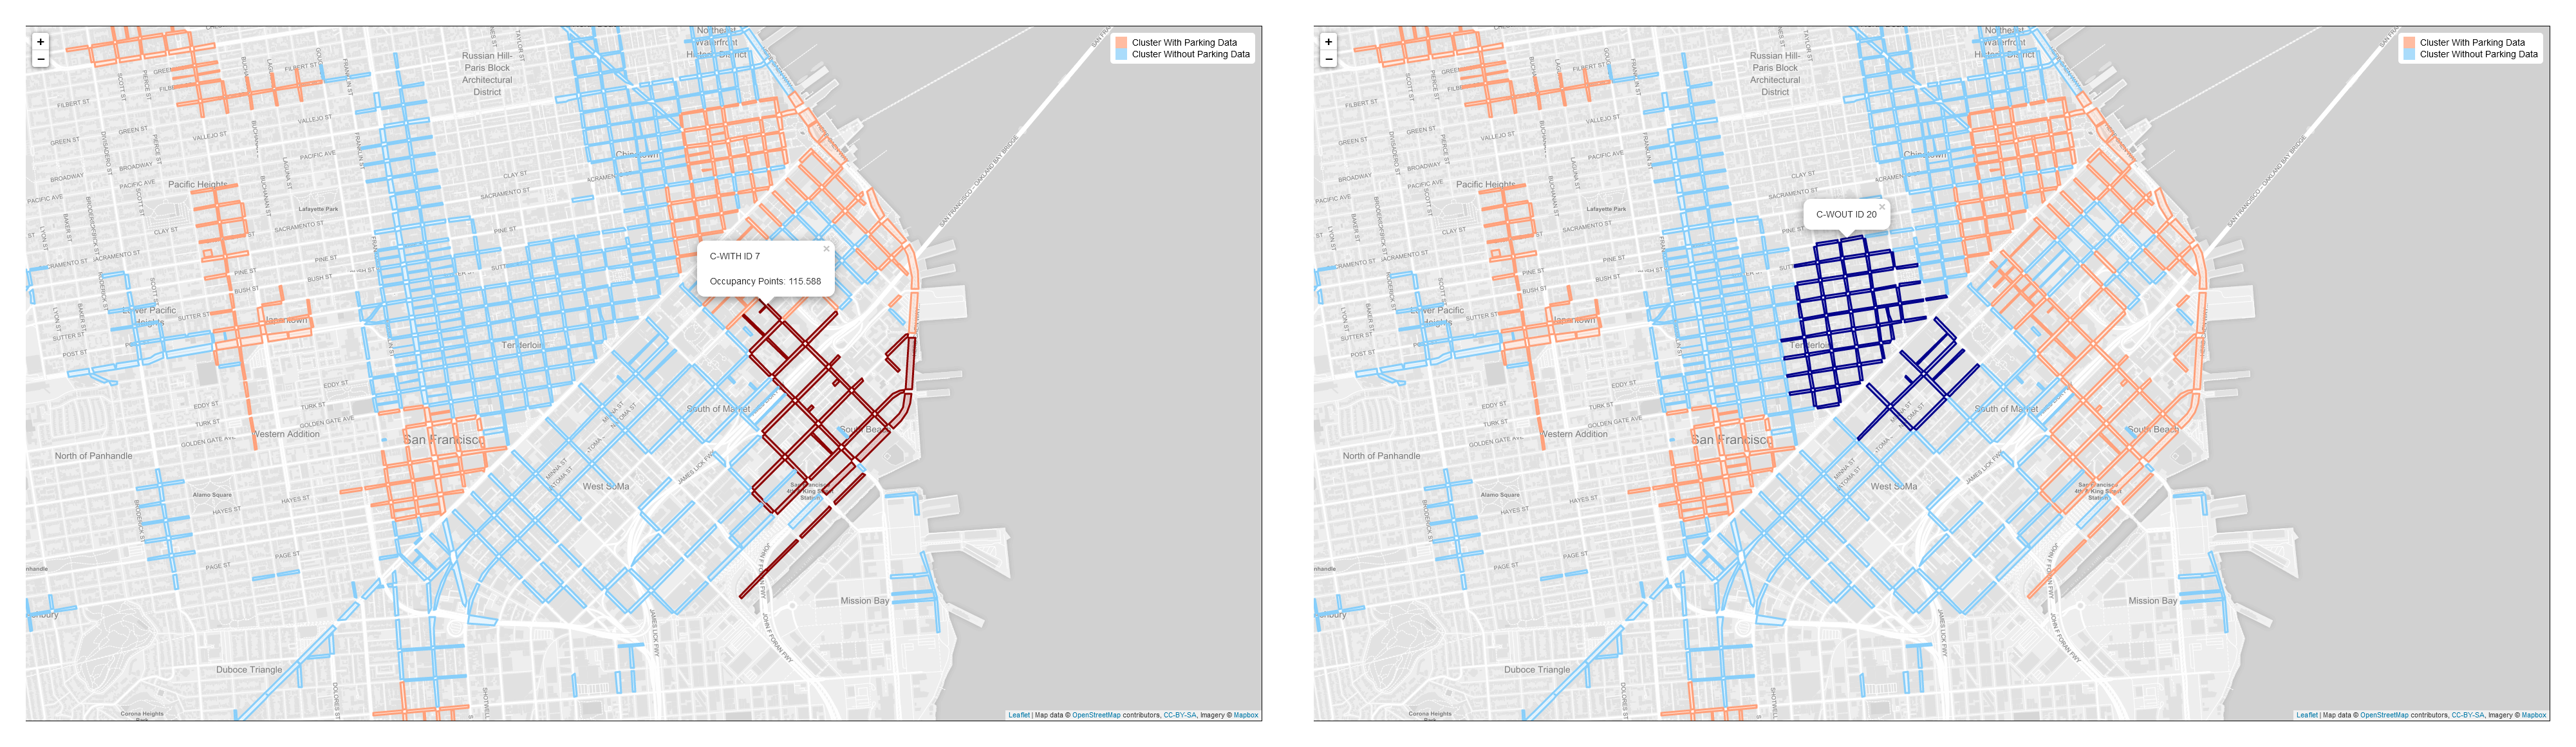
\includegraphics[width=\textwidth]{graphics/highlighted_collage.png}
	\caption{Highlighted cluster \textit{with} parking data on the left side and a cluster \textit{without} parking data on the right side.}
	\label{fig:highlighted_collage}
\end{figure}

The resulting aggregated blocks are worth taking into account when training the machine learning models, as these will average over pieces of information contained in individual blocks. 

\subsection{Similarity functions}
\label{experimental_setup:urban_measure}
Before computing \textit{cluster vectors} and \textit{cluster Gaussians}, we will establish the visiting duration in every amenity.
For this, we use information gathered from Google Places available via Google Maps\footnote{http://maps.google.com}.

We manually collected information from 470 places in San Francisco, for which a maximum duration of stay was provided (the minimum duration is not always given, as indicated earlier).
The data was obtained by manually navigating to every business place and writing the duration visit information in a spreadsheet.
This piece of information is not accessible yet via the Google Places API\footnote{Google Feature Request: \url{https://issuetracker.google.com/issues/35827350}}.
The results are shown in \Cref{tab:amenities_google_places} and the numbers are given in minutes and have been rounded to the nearest integer. We have included only amenities for which at least two stay duration sources were found. 

\begin{table}[!ht]
	\tbl{All amenities listed with their corresponding mean visiting information as collected from Google Places. 
The \emph{cat} column indicates whether the average visiting time is under half an hour (1), 31 to 90 minutes (2), or more than 1.5 hours (3).
}
	%\footnotesize
	{\begin{tabular}{ | l | c | c | c || l | c | c | c |}
		\hline		
		\textbf{amenity name} & \textbf{mean} & \textbf{stdev} & \textbf{cat} & \textbf{amenity name} & \textbf{mean} & \textbf{stdev} & \textbf{cat} \\ \hline
		arts\_centre  & 110 & 37 & 3 & laundry  & 78 & 16 & 2 \\ \hline
		bank  & 42 & 65 & 2 &  library  & 83 & 13 & 2 \\ \hline
		bar  & 121 & 38 & 3 &  music\_school  & 120 & 30 & 3 \\ \hline
		cafe  & 76 & 39 & 2 &  nightclub  & 189 & 20 & 3 \\ \hline
		clinic  & 100 & 29 & 3 &  pharmacy  & 25 & 20 & 1 \\ \hline
		clothes\_store  & 41 & 37 & 2 &  post\_office  & 16 & 2 & 1 \\ \hline
		community\_centre  & 119 & 40 & 3 &  pub  & 135 & 21 & 3 \\ \hline
		dentist  & 104 & 35 & 3 &  restaurant  & 135 & 32 & 3 \\ \hline
		doctors  & 60 & 42 & 2 &  salon  & 141 & 53 & 3 \\ \hline
		embassy  & 75 & 24 & 2 &  shelter  & 90 & 0 & 2 \\ \hline
		fast\_food  & 31 & 15 & 2 &  shop  & 43 & 21 & 2 \\ \hline
		grocery  & 20 & 10 & 1 &  spa  & 161 & 54 & 3 \\ \hline
		gym  & 100 & 22 & 3 &  stripclub  & 140 & 46 & 3 \\ \hline
		hookah\_lounge  & 130 & 17 & 3 &  studio  & 60 & 0 & 2 \\ \hline
		ice\_cream  & 23 & 7 & 1 &  veterinary  & 67 & 29 & 2 \\ \hline
		karaoke  & 188 & 15 & 3 & {\scriptsize vintage\_modern\_resale}  & 38 & 32 & 2 \\ \hline
	\end{tabular}}
	\label{tab:amenities_google_places}
	\begin{tabnote}
		Duration and standard deviation are expressed in minutes. The assigned category for cluster vectors is included.
	\end{tabnote}
\end{table}

Alongside this information, we need the amenity categories in order to derive the \textit{cluster vectors}.
As defined in \Cref{realization:vectors}, the categories are based on the visiting duration mean.
We split them in three categories: 
\begin{romanlist}
	\item under half an hour,
	\item 31 to 90 minutes and
	\item more than 1.5 hours. 
\end{romanlist}
The assigned partitions for every amenity are shown in \Cref{tab:amenities_google_places}. 
The computation of \textit{cluster Gaussians} relies on both the mean and standard deviation of the amenity visiting duration, as defined in \Cref{realization:gaussians}.

\subsection{Amenity area as similarity basis}
\label{experimental_setup:amenity_area}
Together with the similarity functions in \Cref{experimental_setup:urban_measure} we considered \textit{visiting duration} as the basis for creating the urban profile. However, there are other measures that reflect the parking demand towards an amenity, one of them being the area of the particular amenity. OpenStreeMap provides a polygon layer for a certain geographic bounding box, which contains information across all the surfaces in that region (recall \Cref{sec:citydata}). See \Cref{fig:amenity_polygons} for a visualization of the polygons and their areas in OSM. In extracting this information we had two options. 

\begin{figure}[!ht]
	\centering
	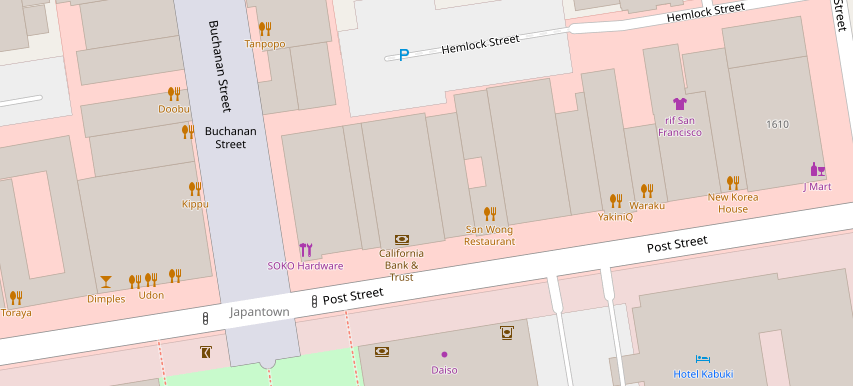
\includegraphics[width=\textwidth]{graphics/amenity_polygons4.png}
	\caption{OSM screenshot emphasizing polygons as buildings and the amenities that are housed by them}
	\label{fig:amenity_polygons}
\end{figure}

Matching the amenities' POIs with the containing OSM polygon and then computing the polygon areas per amenity was the option tried first. This has several drawbacks. The relation POI:polygon is in practice by no means 1:1, i.e. many cases arose where multiple POIs were contained by the same polygon, in which situation the area was split between them; a POI might also be on the edge of several polygons, in which case we have to either (arbitrarily) assign it to the first polygon or to all. The deciding factor against this option was, however, the high \textit{coefficient of variation} for the area values. 

The coefficient of variation (CV) is a measure of dispersion of a probability distribution and is defined as the ratio between the standard deviation and the mean of a sample (cf. Equation \Cref{eq:cv}). When calculating CV based on the matching of POI with the polygons, it came out $2.1$ (value is referenced below).

\begin{equation}
c_v = \frac{\sigma}{\mu} 
\label{eq:cv}
\end{equation}

The other option was to use the \textit{amenity} attribute in the polygon layer for the region. We could avoid the cumbersome matching by leveraging solely the polygon layer and calculating the amenity area mean and its standard deviation. The results are listed in \Cref{tab:amenity_area_values}. On top of that, the coefficient of variation is $0.9$ in this case, significantly lower than before. 

Note that we have reduced the values in the table by a factor of 20, as it turned out that the actual mean and standard deviation were large enough to make the emd Gaussian computation extremely slow. As the standard deviation is linear with regard to the mean, both mean and standard deviation values were reduced conveniently. 

\begin{table}[!ht]
	%\footnotesize
	\tbl{Amenity area values gathered and averaged from OMS polygon layer for the SF\textit{park} region}
	{\begin{tabular}{ | l | c | c | c || l | c | c | c |}
			\hline		
			\textbf{amenity name} & \textbf{mean} & \textbf{stdev} & \textbf{cat} & \textbf{amenity name} & \textbf{mean} & \textbf{stdev} & \textbf{cat} \\ \hline
			arts\_centre & 68 & 60 & 2 & bank & 39 & 20 & 2 \\ \hline
			bar & 19 & 8 & 1 & bicycle\_parking & 8 & 7 & 1 \\ \hline
			biergarten & 11 & 12 & 1 & brokerage & 39 & 9 & 2 \\ \hline
			bus\_station & 588 & 737 & 3 & cafe & 17 & 10 & 1 \\ \hline
			car\_rental & 70 & 43 & 2 & car\_wash & 43 & 48 & 2 \\ \hline
			childcare & 101 & 130 & 3 & cinema & 75 & 43 & 2 \\ \hline
			clinic & 61 & 32 & 2 & community\_centre & 52 & 74 & 2 \\ \hline
			conference\_centre & 401 & 519 & 3 & courthouse & 459 & 201 & 3 \\ \hline
			dentist & 17 & 12 & 1 & doctors & 324 & 568 & 3 \\ \hline
			embassy & 68 & 38 & 2 & fast\_food & 25 & 24 & 1 \\ \hline
			fire\_station & 52 & 27 & 2 & fountain & 24 & 22 & 1 \\ \hline
			fuel & 25 & 27 & 1 & library & 102 & 124 & 3 \\ \hline
			marketplace & 325 & 228 & 3 & music\_rehearsal\_place & 33 & 15 & 1 \\ \hline
			nightclub & 32 & 9 & 1 & nursing\_home & 97 & 47 & 2 \\ \hline
			parking & 182 & 309 & 3 & pharmacy & 65 & 38 & 2 \\ \hline
			place\_of\_worship & 60 & 62 & 2 & police & 137 & 124 & 3 \\ \hline
			post\_office & 39 & 11 & 2 & pub & 25 & 25 & 1 \\ \hline
			public\_building & 280 & 236 & 3 & recycling & 28 & 20 & 1 \\ \hline
			restaurant & 22 & 16 & 1 & school & 740 & 1280 & 3 \\ \hline
			social\_centre & 30 & 21 & 1 & social\_facility & 356 & 801 & 3 \\ \hline
			stripclub & 50 & 10 & 2 & studio & 268 & 307 & 3 \\ \hline
			swimming\_pool & 16 & 9 & 1 & swingerclub & 27 & 4 & 1 \\ \hline
			theatre & 174 & 191 & 3 & toilets & 7 & 5 & 1 \\ \hline
			training & 72 & 94 & 2 & veterinary & 21 & 7 & 1 \\ \hline
	\end{tabular}}
	\label{tab:amenity_area_values}
	\begin{tabnote}
		The mean and standard deviation values were reduced by a 20x factor. The categories for cosine vectors are 0 - 35, 36 - 100, 100+.
	\end{tabnote}
\end{table}

\subsection{Model training and evaluation for clusters \emph{with} parking data}
\label{experimental_setup:model_training}
%We use four methods to train models for the clusters \textit{with} parking data: \textit{decision trees}, \textit{support vector machines}, \textit{multilayer perceptrons}, \textit{gradient boosted trees}. 
As training data, the SF\textit{park} \textit{occupancy data} is used with \textit{street blocks} as location unit. It turns out that training on the additional SF\textit{park} data, i.e., traffic and events, encounters some problems. 

The \textit{traffic data} do not share the same location unit with the parking occupancy's street block. Even when aggregating traffic data on the district level, which is available for the occupancy data as well, it does not prove an additional value to the training. 

For the SF\textit{park} \textit{events data} we encounter the same problem as for the traffic data: the location unit does not match the block. In fact, the events are marked for streets, whose association to blocks is not determinable. 

\textit{Parking revenue data} is provided for districts, which again are too general to make a difference in training.

Finally, \textit{weather data} and \textit{fuel data} are given per city, hence making even less an impact to improve the model.  

\subsection{Aggregating training data}
\label{experimental_setup:aggregating_training_data}
As indicated in \Cref{realization:machine_learning_models}, the training data is aggregated across all blocks so that it becomes comparable to other clusters and can be used in training and testing models. The averaging is performed per timestamp, i.e., if multiple blocks have an occupancy record for the same time and block, the occupancy rate will be averaged for both of these. Features such as \textit{price} and \textit{parking capacity per block} are averaged as well. See \Cref{tab:aggregating_datapoints} for an example of this process. This means that the original collection of data records shrinks, which should decrease the training time. In \Cref{tab:models_training_points}, the expansion/shrinking rate is shown for various number of clusters.

\begin{table}
	%\footnotesize
	\tbl{Example of aggregating datapoints}
	{\begin{tabular}{ c }
			\begin{tabular}{ | c | c | c | c | c |}
				\hline
				\textbf{block id} & \textbf{timestamp} & \textbf{price rate} & \textbf{total spots} & \textbf{occupied} \\ \hline
				902   & {2011-04-02 7:00:00} & 0 & 46 & 58 \\ \hline
				32800 & {2011-04-02 7:00:00} & 0 & 32 & 2 \\ \hline
				33005 & {2011-04-02 7:00:00} & 3 & 36 & 12 \\ \hline
				902   & {2011-04-02 8:00:00} & 2 & 46 & 54 \\ \hline
				32800 & {2011-04-02 8:00:00} & 4 & 32 & 5 \\ \hline
				33005 & {2011-04-02 8:00:00} & 3 & 36 & 22 \\ \hline
			\end{tabular} \\
			%\vskip 0.2cm
			%\\
			\colrule
			%\vskip 0.2cm
			%\\
			%\hskip 1.8cm
			\begin{tabular}{ | c | c | c | c |}
				\hline
				\textbf{timestamp} & \textbf{price rate} & \textbf{total spots} & \textbf{occupied} \\ \hline
				{2011-04-02 7:00:00} & \textbf{1} & \textbf{38} & \textbf{24} \\ \hline
				{2011-04-02 8:00:00} & \textbf{3} & \textbf{38} & \textbf{27} \\ \hline
			\end{tabular}
	\end{tabular}}
	\begin{tabnote}
		In the subtable above, three distinct blocks belonging to a cluster are transformed into two entries by averaging \textit{price rate}, \textit{total spots} and \textit{occupied} attributes for the two distinct timestamps (subtable below)
	\end{tabnote}
	\label{tab:aggregating_datapoints}
\end{table}

%\begin{table}[!ht]
%	\setlength\extrarowheight{5pt}
%	\centering
%	\footnotesize
%	\begin{tabular}{| c | S[table-format=5.0] | S[table-format=6] | S[table-format=2.1] |}
%		\hline
%		\textbf{Cluster ID} & \textbf{Data Points} & \textbf{Occupancy Points} & \textbf{\begin{tabular}{@{}c@{}}Blocks\\per Timestamp\end{tabular}} \\ \hline
%		0 & 9879 & 120320 & 12.2 \\ \hline
%		1 & 12387 & 203728 & 16.4 \\ \hline
%		2 & 8713 & 61839 & 7.1 \\ \hline
%		3 & 6134 & 22371 & 3.6 \\ \hline
%		4 & 9586 & 110463 & 11.5 \\ \hline
%		5 & 9112 & 87316 & 9.6 \\ \hline
%		6 & 10244 & 118096 & 11.5 \\ \hline
%		7 & 9500 & 115588 & 12.2 \\ \hline
%		8 & 9051 & 112245 & 12.4 \\ \hline
%		9 & 8713 & 76230 & 8.7 \\ \hline
%		\textbf{Average}	& 9332 & 102820 & 10.5 \\ \hline
%	\end{tabular}
%	\captionsetup{justification=centering}
%	\caption{Number of training points per model alongside the initial occupancy points within the containing blocks.}
%	\label{tab:models_training_points}
%\end{table}

\begin{table}[!ht]
		%\setlength\extrarowheight{5pt}
		%\centering
		%\footnotesize
		\tbl{Number of datapoints aggregated per timestamp vs. all datapoints alongside the shrinking rate for 8, 16 and 32 clusters}
		{\begin{tabular}{ | c | c | c | c | } %| c | S[table-format=5.0] | S[table-format=6] | S[table-format=2.1] |
			\hline
			{cluster size} & {aggregated datapoints} & {all datapoints} & {shrinking/expansion rate} \\ \hline
			8 &	9741 & 128525 &	12.3 \\ \hline
			16 & 8409 &	73332 &	8.3 \\ \hline
			32 & 6257 &	29355 &	4.6 \\ \hline
		\end{tabular}}
		\begin{tabnote}
			Values have been averaged across clusters
		\end{tabnote}
		%\captionsetup{justification=centering}
		\label{tab:models_training_points}
\end{table}

%\subsection{Model Evaluation for Clusters \textit{with} Parking Data}
%\label{evaluation:training_testing_errors}
In \Cref{fig:cwith} a screenshot of the web application showing a sample of the results is illustrated. \Cref{fig:cwith_table} displays the presented table in more detail.

\begin{figure}[!ht]
	\centering
	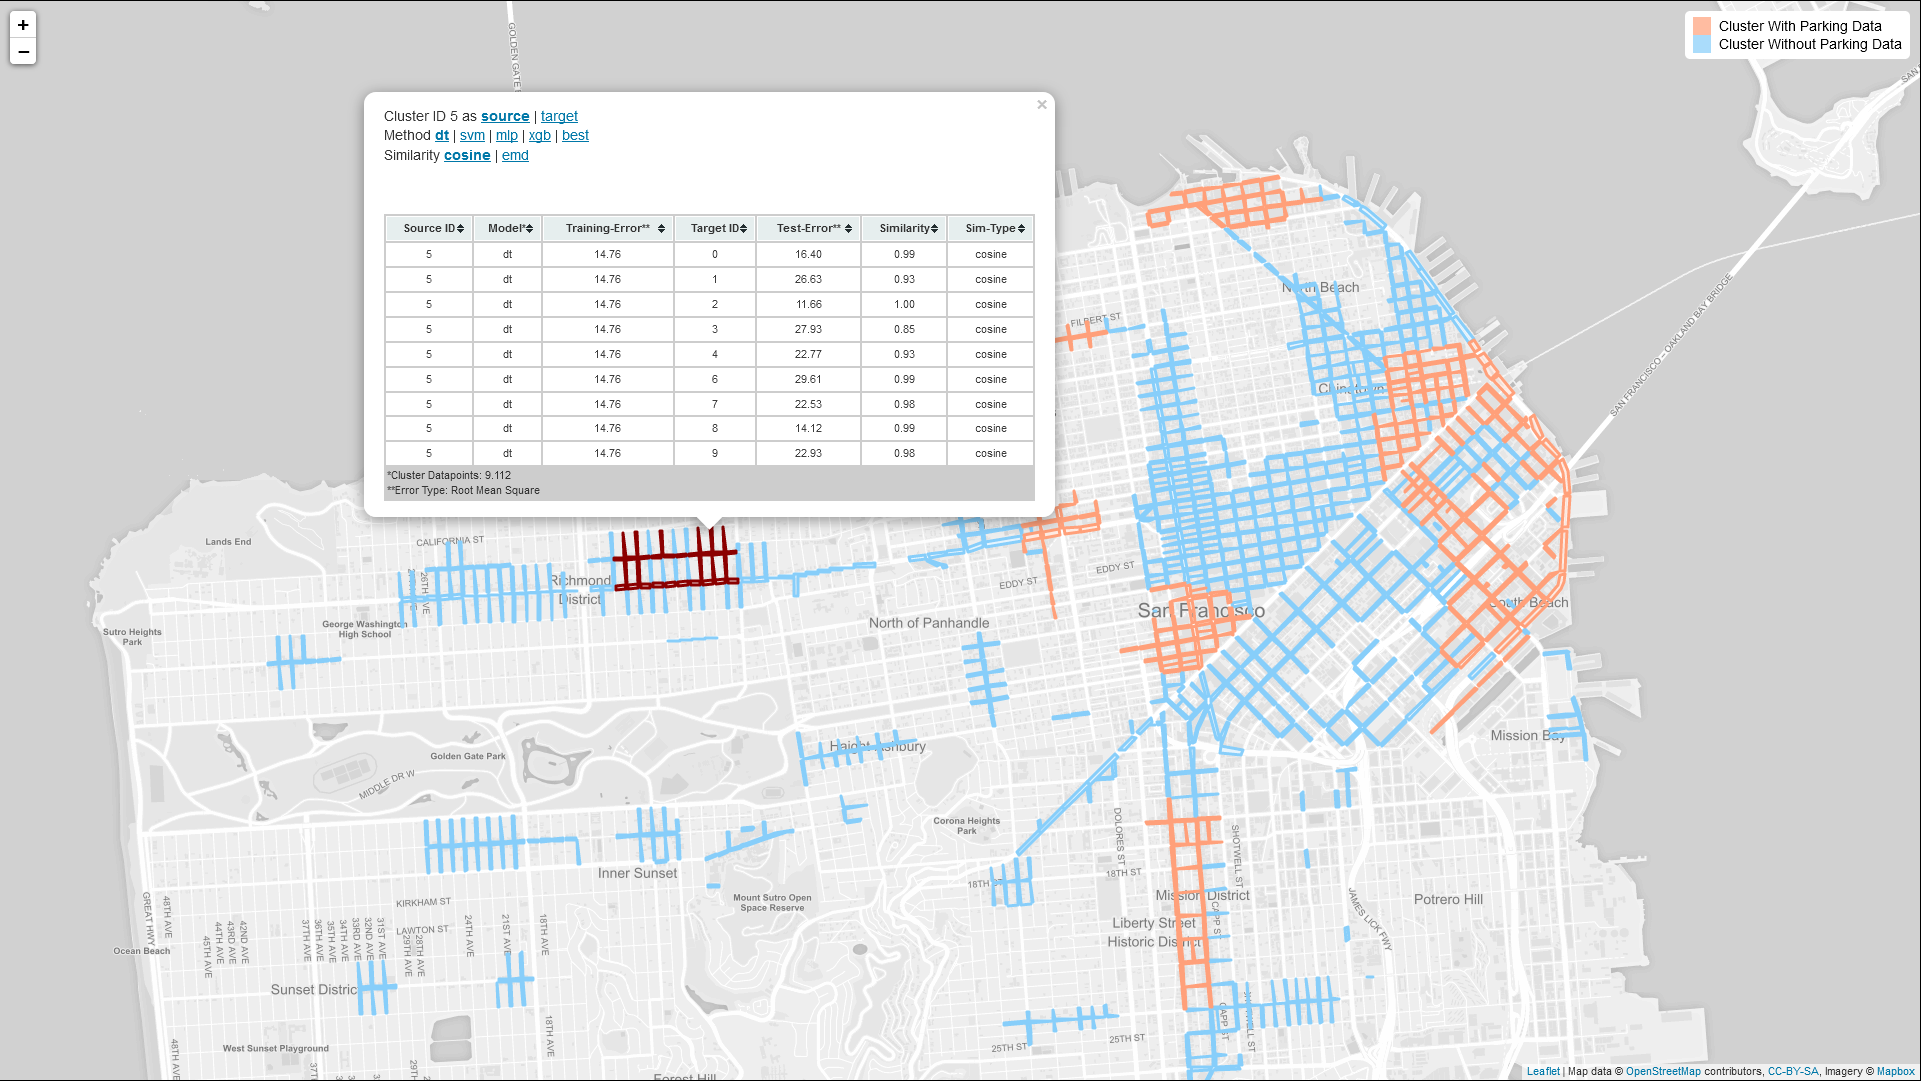
\includegraphics[width=0.8\textwidth]{graphics/cwith_source_dt_cosine.png}
	\caption{Selected cluster \textit{with} parking data and the pop-up table in the Leaflet application.}
	\label{fig:cwith}
\end{figure}

\begin{figure}[!ht]
	\centering
	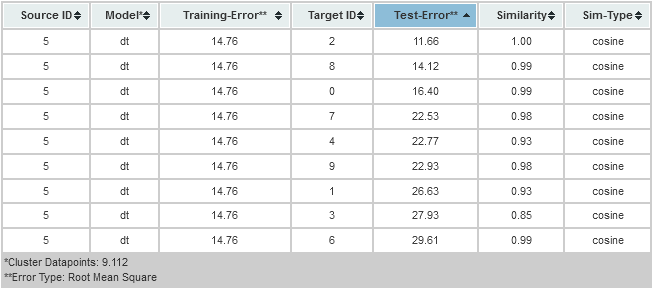
\includegraphics[width=0.8\textwidth]{graphics/cwith_source_dt_cosine_table.png}
	\caption{The pop-up table for the Leaflet application view of \Cref{fig:cwith}.}
	\label{fig:cwith_table}
\end{figure}

\section{Evaluation}
We shall evaluate various pieces of the system that has been presented. Firstly, in \Cref{evaluation:best_model}, we shall establish the machine learning method that achieves best results on average across clusters. 

\Cref{evaluation:similarity_vs_estimation_sec} is the heart of the evaluation. It consists in comparing the cluster models' test error with the independently-computed similarity values between clusters. More specifically, a \textit{source} cluster's model will tested on a \textit{target} cluster and the error is correlated to the similarity between the \textit{source} and the \textit{target} clusters. Both \textit{cosine} and \textit{emd} functions will be used. The correlations will be expressed as Pearson- and Spearman's rank coefficients.

In the following \Cref{evaluation:estimations_cwout}, we take a look at the results of applying the models to clusters \textit{without parking data} and show screenshots from the concrete web application. \Cref{evaluation:entire_datapoints} looks at the model test errors and correlation results by skipping the aggregating step in machine learning training, i.e. instead of averaging the datapoints over timestamp per cluster, we build the cluster models using the entire occupancy data. 

\Cref{evaluation:amenity_area} follows up on \Cref{experimental_setup:amenity_area} and uses the \textit{amenity area} as the basis for the similarity functions in calculating the correlations between model test errors and similarity values. Finally, in \Cref{evaluation:machine_learning_better} we question whether the similarity function approach is the most efficient and transfer its purpose to the machine learning phrase. The model will receive absolute \textit{cosine} and \textit{emd Gaussian} values as additional features and its model test error and correlation values will be compared to the ones from the original approach.

\subsection{Best Model Method}
\label{evaluation:best_model}
Models were trained using four methods: decision trees, support vector machines, multilayer perceptrons, gradient boosted trees. \Cref{evaluation:best_model_method} shows the distribution of best machine learning methods in case of 8 and 16 clusters.
The values were obtained by summing up the number of times a method produced the least estimation error, i.e., RMSE, among the four methods for all combinations of clusters with parking data $(\mathcal{C}_{source}, \mathcal{C}_{target})$.
Extreme gradient boosting claims the first spot in both cases.

For further experiments in the evaluation we shall train the models exclusively with extreme gradient boosting.

\begin{table}[!ht]
	%\centering
	%\small
	%\setlength\extrarowheight{5pt}
	\tbl{The proportion of best models among decision trees, support vector machine, multilayer perceptron and gradient boosting  measured as RMSE when applied on all pairs of clusters}
	{\begin{tabular}{ | c | c | c | c | c |}
		\hline
		& \textbf{dt} & \textbf{svm} & \textbf{mlp} & \textbf{xgb} \\ \hline
		\textbf{8 clusters} & 24.6\% & 17.5\% & 12.3\% & \textbf{45.6\%} \\ \hline
		\textbf{16 clusters} & 14.6\% & 13.8\% & 13.8\% & \textbf{57.9\%} \\ \hline
	\end{tabular}}
\label{evaluation:best_model_method}
\end{table}

%\subsection{Clustered- vs. Total Models}
%\label{experimental_setup:total_models}
%One assumption of our approach is that models originating from smaller clusters are better at predicting occupancy than models trained with the entire city area.
%We have compared the two types of models during our tests.
%For each target cluster $\mathcal{C}_{target}$, we determine the source cluster $\mathcal{C}_{source}$ whose model has the best estimation error when applied on $\mathcal{C}_{target}$.
%We also train a model containing the entire city area with parking data $\mathcal{A}$ minus $\mathcal{C}_{target}$'s data and compute this model's estimation error on $\mathcal{C}_{target}$.
%As we can observe from \Cref{evaluation:cluster_vs_total_8c}, in the case of 8 clusters, and in \Cref{evaluation:cluster_vs_total_16c} for 16 clusters, the cluster's models estimations are superior to the ones of the total model with very few exceptions.

%\begin{table}[!ht]
%	%\centering
%	%\scriptsize
%	%\setlength\extrarowheight{5pt}
%	\tbl{Comparison between the estimations of the total models versus the ones of clustered models, in case the city is split into 8 clusters. Errors are expressed as RMSE.}
%	{\begin{tabular}{ | c | c | c | c | c | c |}
%		\hline
%		$\mathcal{C}_{target}$ & $\mathcal{M}(\mathcal{A} \setminus \mathcal{C}_{target})$ & $error_{total}$ & $error_{cluster}$ & $\mathcal{M}(\mathcal{C}_{source})$ & $\mathcal{C}_{source}$ \\ \hline
%		0 & xgb & 18.20 & 16.10 & xgb & 6 \\ \hline
%		1 & dt & 17.44 & 12.14 & xgb & 7 \\ \hline
%		2 & xgb & 20.33 & 17.45 & svm & 5 \\ \hline
%		3 &	xgb & 17.59 & 13.35 & xgb &	1 \\ \hline
%		4 & dt & 17.49 & 17.30 & xgb & 6 \\ \hline
%		5 & xgb & 18.44 & 16.08 & xgb &	2 \\ \hline
%		6 & xgb & 16.00 & 15.92 & svm &	0 \\ \hline
%		7 & dt & 16.38 & 10.87 & xgb & 3 \\ \hline
%	\end{tabular}}
%	\label{evaluation:cluster_vs_total_8c}
%\end{table}

%\begin{table}[!ht]
%	%\centering
%	%\scriptsize
%	%\setlength\extrarowheight{5pt}
%	\tbl{Comparison between the estimations of the total model versus the ones of clustered models, in case the city is split into 16 clusters. Errors are expressed as RMSE.}
%	{\begin{tabular}{ | c | c | c | c | c | c |}
%		\hline
%		$\mathcal{C}_{target}$ & $\mathcal{M}(\mathcal{A} \setminus \mathcal{C}_{target})$ & $error_{total}$ & $error_{cluster}$ & $\mathcal{M}(\mathcal{C}_{source})$ & $\mathcal{C}_{source}$ \\ \hline
%		0 & mlp & 19.53 & 13.40 & xgb &	15 \\ \hline
%		1 & xgb & 17.82 & 17.18 & xgb &	7 \\ \hline
%		2 &	xgb & 20.79 & 17.97 & svm &	6 \\ \hline
%		3 & xgb & 16.44 & 13.25 & xgb &	0 \\ \hline
%		4 & xgb & 17.58 & 16.40 & xgb & 8 \\ \hline
%		5 & dt & 17.59 & 10.93 & xgb & 0 \\ \hline
%		6 & xgb & 18.44 & 16.29 & xgb & 2 \\ \hline
%		7 & xgb & 16.73 & 16.38 & xgb & 9 \\ \hline
%		8 & xgb & 13.57 & 14.14 & xgb & 10 \\ \hline
%		9 & xgb & 16.90 & 15.95 & xgb & 10 \\ \hline
%		10 & xgb & 16.25 & 16.45 & xgb & 7 \\ \hline
%		11 & mlp & 21.73 & 14.95 & xgb & 11 \\ \hline
%		12 & xgb & 20.33 & 15.42 & xgb & 0 \\ \hline
%		13 & dt & 14.52 & 11.39 & xgb & 15 \\ \hline
%		14 & dt & 22.93 & 18.73 & svm & 6 \\ \hline
%		15 & dt & 20.63 & 13.33 & xgb & 0 \\ \hline
%	\end{tabular}}
%	\label{evaluation:cluster_vs_total_16c}
%\end{table}

\subsection{Similarity Values vs. Estimation Errors}
\label{evaluation:similarity_vs_estimation_sec}
The central goal of this work is estimate the occupancy for clusters where no parking data is available using model predictions and pair-wise cluster similarity values. If the model prediction accuracy can be measured on clusters with parking data by means of their test errors, we still need to show that the cluster similarity values express indeed a similarity of occupancy. We shall use clusters with parking data to check this and use the model predictions as occupancy references: the higher the absolute correlation between the cluster similarity values and the model test errors, the better the accuracy of the cluster similarity. Concretely, for every pair of clusters ($\mathcal{C}_{source}, \mathcal{C}_{target}$) a model $\mathcal{M}_{\mathcal{C}_{source}}$ is trained on $\mathcal{C}_{source}$ and its test prediction error on $\mathcal{M}_{\mathcal{C}_{source}}(\mathcal{C}_{target})$ shall be correlated with the cosine and emd similarity values between $\mathcal{C}_{source}$ and $\mathcal{C}_{target}$. Here we use two correlation coefficients: the Pearson correlation coefficient and Spearman's rank correlation coefficient, resulting in four correlation measures: 
\begin{romanlist}
	\item	cosine (Pearson) correlation
	\item 	cosine (Spearman's) rank correlation
	\item 	emd (Pearson) correlation
	\item 	emd (Spearman's) rank correlation. 
\end{romanlist}
The evaluation was performed for configurations of 8 and respectively 16 clusters. Additionally, we varied the \textit{merge distance} to see how the correlation behaves. The similarity values are hence calculated for 100m, 200m, and 400m merge distance respectively. In \Cref{tab:similarity_vs_estimation} the final results are shown. For each correlation measure (\textit{cosine}, \textit{rank cosine}, \textit{emd}, \textit{rank emd}) the value is averaged across all clusters. Due to their mathematical meaning explained in \Cref{realization:similarity_functions}, for cosine measure a negative correlation is optimal, whereas for emd a positive correlation value is beneficial. The models taken were trained with gradient boosted trees. 
	
We notice that the cosine similarity achieves better results than emd for the same testing configuration, peaking for 8 clusters and 100m merge distance. Its average Pearson coefficient is $-0.55$, while the mean Spearman rank coefficient is $-0.49$. emd positively correlates the most for the same testing configuration (8 clusters, 100m), when the average Pearson coefficient is at $0.28$ and Spearman's rank coefficient equals $0.23$. There is a clear descending trend in correlations, as the merge distance increases.  Also, the results for 8 clusters are superior to the ones when the city is split in 16 clusters. 

Further in the evaluation runs we shall fix the merge distance to 100m.

\begin{table}[!ht]
		%\centering
		%\small
		%\setlength\extrarowheight{5pt}
		%\resizebox{\textwidth}{!}{
		\tbl{Correlations between similarity values and model estimations errors for pairs of clusters \textit{with} parking data ($\mathcal{C}_{source}, \mathcal{C}_{target})$.}
		{\begin{tabular}{ | c | c | c | c | c | c | c | c | c |}
			\hline
			{} & \multicolumn{4}{c|}{8 clusters} \\ \hline
			{merge distance} & cosine & rank\_cosine & emd & rank\_emd \\ \hline
			100m & \textbf{-0.55} & \textbf{-0.49} & \textbf{0.28} & 0.23 \\ \hline
			%100m & \textbf{100\%} & \textbf{100\%} & \textbf{87.5\%} & \textbf{75\%} \\ \hline
			200m & -0.34 & -0.30 & 0.26	& 0.23 \\ \hline
			%200m & 75\% & 75\% & 75\% & 75\% \\ \hline
			400m & -0.23 & -0.08 & 0.25 & \textbf{0.27} \\ \hline
			%400m & 62.5\% & 50\% & 75\% & 75\% \\ \hline
		\end{tabular}}
		\vspace{3em}
		{\begin{tabular}{ | c | c | c | c | c | }
			\hline
			{} & \multicolumn{4}{c|}{16 clusters} \\ \hline
			{merge distance} & cosine & rank\_cosine & emd & rank\_emd \\ \hline
			100m & \textbf{-0.20} & \textbf{-0.17} & \textbf{0.10} & \textbf{0.11} \\ \hline
			%100m & 75\% & 75\% & 68.75\% & 62.5\% \\ \hline
			200m & -0.13 & -0.11 & 0.02 & 0.02 \\ \hline
			%200m & 75\% & 75\% & 56.3\% & 56.3\% \\ \hline
			400m & -0.17 & -0.17 & 0.08 & 0.11 \\ \hline
			%400m & 68.8\% & 68.8\% & 62.5\% & 62.5\% \\ \hline
		\end{tabular}}
		\label{tab:similarity_vs_estimation}
		\begin{tabnote}
			For cosine similarity the values show a negative correlation tendency, while for the correlation based on emd similarity expresses a positive correlation tendency. The correlations are measured using Pearson coefficient and Spearman's rank coefficient.
		\end{tabnote}
\end{table}	

\subsection{Estimations for Clusters \textit{without} Parking Data}
\label{evaluation:estimations_cwout}
We apply the models trained on SF\textit{park} data on clusters \textit{without} parking data.
The testing data records are composed of values equal to the averages of the respective data types in all clusters \textit{with} parking data.
This is the case for \textit{parking price} and \textit{parking capacity}.
One piece of data that still needs to be provided so that the estimation is computed is the date and time.
For convenience, we choose the next day at the point when the user starts the model training. 
An example of the estimation is visualized \Cref{fig:cwout_table}.

\begin{figure}[!ht]
	\centering
	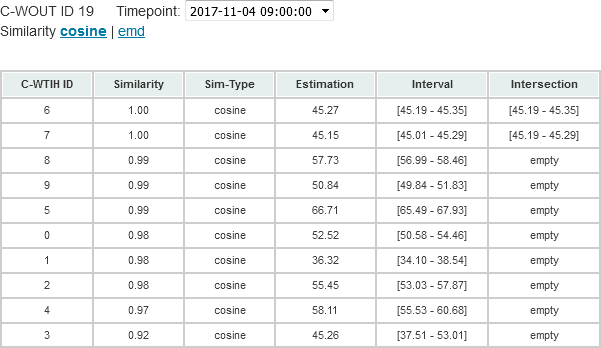
\includegraphics[width=0.8\textwidth]{graphics/cwout_cosine_table.png}
	\caption{The pop-up table of a cluster without data.
		Notice the drop-down list from which the time can be selected.}
	\label{fig:cwout_table}
\end{figure}

%\section{Extensions}
%\label{extensions}
%Up to this point it was our goal to show that the approach involving clustering and similarity improves upon the simple machine learning approach. 
%In the following we present some extensions and variations that consolidate the approach presented, if not improve upon it. 

%Furthermore, we added a configuration with 32 clusters on which we tested or hypotheses.

\subsection{Models built on all occupancy datapoints}
\label{evaluation:entire_datapoints}
Up to now, the evaluation involved models trained and tested on aggregated datapoints, as explained in \Cref{experimental_setup:aggregating_training_data}. We ask ourselves however, whether a model trained on all datapoints performs better when tested on an aggregated cluster. Or whether an aggregate model deliver better results on an all-datapoints cluster than a model trained on all datapoints? Here we experiment these combinations by training models on both all- and aggregate datapoints and apply them on both types of aggregation forms. 

See \Cref{tab:train_test_errors} for an overview of test errors for 8 and 16 clusters. One observes that the errors from models applied on aggregated datapoints are about 5 unit points (=5\%) smaller than the errors from models applied on all datapoints. This is naturally accounted for by the smaller spread of occupancy values that the aggregation brings with itself. As far as source models are concerned, there is no significant difference between the aggregate and all datapoint models, i.e. the margin is under 1\%.

In \Cref{tab:correlation_values} the resulting correlations of testing errors with cosine- and emd similarity values are listed for models of 8 and 16 cluster configurations. Regarding the number of clusters, the values for 8-cluster models are clearly superior to the 16-cluster models. When comparing by target datapoints type, the models applied on aggregated datapoints have a slight edge, with the cosine- and rank cosine correlation values being on average closer to -1 and emd- and rank emd correlation values being closer to 1. However, for 16 clusters the correlations tendency is barely noticeable.
	
\begin{table}[!ht]
	%\centering
	%\small
	\tbl{Test error for ML models build alternatively with all- and aggregated datapoints}
	%\setlength\extrarowheight{5pt}
	%\resizebox{\textwidth}{!}{
	{\begin{tabular}{ | c | c | c | c | c | c | }
		\hline
		{cluster size} & {datapoints source} & {datapoints target} & {test error} \\ \hline
		8	&	aggregate 	&	aggregate 	& 	\textbf{20.19} 	\\ \hline
		8	&	all 		&	aggregate 	& 	21.37	\\ \hline \hline
		8	&	aggregate 	&	all 		& 	26.25	\\ \hline
		8	&	all			& 	all 		&	26.68	\\ \hline \hline
		16	&	aggregate	& 	aggregate 	&	\textbf{20.47}	\\ \hline
		16	&	all			& 	aggregate 	& 	21.32	\\ \hline \hline
		16	&	aggregate	& 	all 		& 	25.97	\\ \hline
		16	&	all			&	all 		&	26.52	\\ \hline \hline
	\end{tabular}}
	\label{tab:train_test_errors}
	\begin{tabnote}
		Test errors for the same number of clusters can be accurately compared when the \textit{datapoints target} is the same. All models above were build using extreme gradient boosting.
	\end{tabnote}
\end{table}
	
\begin{table}[!ht]
	%\centering
	%\small
	%\setlength\extrarowheight{5pt}
	%\resizebox{\textwidth}{!}{
	\tbl{Resulting correlation values for ML models built using all- and aggregated datapoints}
	{\begin{tabular}{ | c | c | c | c | c | c | c | }
		\hline
		{cluster size} & {datapoints source} & {datapoints target} & cosine & rank\_cosine & emd & rank\_emd \\ \hline
		8	&	aggregate 	&	aggregate 	& 	\textbf{-0.53}	&	\textbf{-0.52}	&	0.30	&	0.17 	\\ \hline
		8	&	all 		&	aggregate 	& 	-0.53	&	-0.43	&	\textbf{0.37}	&	\textbf{0.27}	\\ \hline \hline
		8	&	aggregate 	&	all 		& 	-0.35	&	-0.36	&	0.20	&	0.14	\\ \hline
		8	&	all			& 	all 		&	-0.41	&	-0.43	&	0.34	&	0.25	\\ \hline \hline
		16	&	aggregate	& 	aggregate 	&	-0.16	&	-0.11	&	0.10	&	0.05	\\ \hline
		16	&	all			& 	aggregate 	& 	\textbf{-0.18}	&	\textbf{-0.17}	&	\textbf{0.22}	&	\textbf{0.17}	\\ \hline \hline
		16	&	aggregate	& 	all 		& 	-0.09	&	-0.06	&	0.08	&	0.00	\\ \hline
		16	&	all			&	all 		&	-0.10	&	-0.11	&	0.17	&	0.08	\\ \hline \hline
	\end{tabular}}
	\label{tab:correlation_values}
	\begin{tabnote}
		All models above were build using extreme gradient boosting.
	\end{tabnote}
\end{table}
	
	
\subsection{Amenity area as similarity basis}
\label{extensions:amenity_area}
Together with the similarity functions we considered \textit{timespent} as the basis for creating the urban profile (recall \ref{experimental_setup:urban_measure}). However, there are other measures that reflect the parking demand corresponding towards an amenity, one of them being area of the particular amenity, which is available in OpenStreetMap. OSM provides a \textit{polygon layer} for a certain geographic bounding box, which contains information across all the surfaces in that region (recall \ref{sec:citydata}). In extracting this information we had two options. 

\subsection{Amenity area results}
\label{evaluation:amenity_area}
Following up on \Cref{experimental_setup:amenity_area} and taking \textit{amenity area} as the basis for the cosine- and emd similarity values leads in practice to correlations listed in \Cref{tab:correlation_amenity_area} for 8- and 16 cluster configurations. The superiority of the correlation values using \textit{visiting duration} is observed both for cosine- and rank cosine correlations, which are closer to -1, and for the emd- and rank emd correlations, which are nearer to 1. All correlation values for 16 clusters are, however, relatively weak in absolute measures.

\begin{table}[!ht]
		%\centering
		%\small
		%\setlength\extrarowheight{5pt}
		%\resizebox{\textwidth}{!}{
		\tbl{The correlation results computed using similarity values based on \textit{amenity area}. }
		{\begin{tabular}{ | c | c | c | c | c | c | c | }
			\hline
			{cluster size} 	& {amenity type} 	& datapoints (train/test) 	& cosine 	& rank\_cosine & emd & rank\_emd \\ \hline
			8 				& {visiting duration} 		& agg/agg 		& \textbf{-0.53}	& \textbf{-0.52}		&	\textbf{0.30}	&	\textbf{0.17} \\ \hline
			8 				& area 				& agg/agg 		& 0.05	&	0.11	&	0.14	&	0.22 \\ \hline \hline
			16 				& {visiting duration} 		& agg/agg 		& -0.16	&	-0.11	&	0.10	&	0.05 \\ \hline
			16 				& area 				& agg/agg 		& -0.09	&	-0.03	&	0.09	&	0.07 \\ \hline
		\end{tabular}}
		\begin{tabnote}
			All models above were build using extreme gradient boosting, trained and tested on aggregated datapoints.  
		\end{tabnote}
		\label{tab:correlation_amenity_area}
\end{table}

\subsection{Extended prediction models}
\label{evaluation:machine_learning_better}
An alternative to building urban measures and similarity functions is to let machine learning figure out the similarities by itself. One can simply add the city data as further training information for clusters. The purpose is to produce better predictions by leveraging unknown patterns in the city data. Hence, features representing the \textit{cosine} and \textit{emd} functions are added to the model, as follows: 
\begin{romanlist}
	\item k features corresponding to the k categories the amenities are split in, i.e. the magnitudes of the vectors for each category;
	\item a feature corresponding to the emd Gaussian value for that cluster, loosely interpreted as the "total accumulated visiting duration" for that cluster, in case of \textit{visiting duration}, or the "total accumulated area" among all amenities in that cluster, for the amenity area; mathematically it is expressed in Equation \Cref{eq:emd_gaussian_magnitude}
	\begin{equation}
		feature(emd)=x \cdot f(x)
		\label{eq:emd_gaussian_magnitude}
	\end{equation}
	{\centering
	where $x$ = 
	$
	\begin{dcases}
	\text{duration in minutes}, & \text{if similarity is \textit{amenity visiting duration}} \\
	\text{area in square meters}, & \text{if similarity is \textit{amenity area}}.
	\end{dcases}
	$ \\
	and $f$ is the constructed emd Gaussian function that equals the number of amenities in the cluster for any value x.}
\end{romanlist}

We subsequently build \textit{extended machine learning models} that additionally contain the features above. Since these features are identical for all datapoints in a cluster, the model needs to be trained on multiple clusters. Therefore, models on $n-1$ out of $n$ clusters will be build and tested on the remaining cluster. These \textit{all-but-one} or \textit{total models} will be constructed for all $n$ combinations of $n-1$ clusters and their averaged test errors will compared to total models that contain the normal features. The resulting test errors are shown in \Cref{tab:extended_models_comparison} for various number of clusters. 

With one single exception the simple total models achieve a better prediction performance, meaning that the addition of the two features did not help with finding better parking occupancy values for the test clusters.

\begin{table}[!ht]
	%\footnotesize
	\tbl{Total models extended with cosine and emd features compared to total models with the previous feature set}
	{\begin{tabular}{ | c | c | c | c | }
		\hline		
		\textbf{cluster size}  & \textbf{model} & \textbf{test error average} \\ \hline
		4 & {xgb} & \textbf{14.92} \\ \hline
		4 & {xgb extended} & 16.18 \\ \hline \hline
		8 & {xgb} & \textbf{18.12} \\ \hline
		8 & {xgb extended} & 19.58 \\ \hline \hline
		%8 & {dt} & \textbf{18.85} & \textbf{18.52} \\ \hline
		%8 & {dt extended} & 19.84 & 19.46 \\ \hline \hline
		%8 & {svm} & TBD & TBD \\ \hline
		%8 & {svm extended} & 20.15 & 23.62 \\ \hline
		%8 & {mlp} & TBD & TBD \\ \hline
		%8 & {mlp extended} & 54.62 & 203.22 \\ \hline
		16 & {xgb} & 18.19 \\ \hline
		16 & {xgb extended} & \textbf{18.09} \\ \hline \hline
		%16 & {dt} & 19.14 & 18.83 \\ \hline
		%16 & {dt extended} & \textbf{18.77} & \textbf{17.81} \\ \hline
		%16 & {svm} & TBD & TBD \\ \hline
		%16 & {svm extended} & 22.52 & 23.49 \\ \hline
		%16 & {mlp} & TBD & TBD \\ \hline
		%16 & {mlp extended} & 22.53	& 19.36 \\ \hline
		32 & {xgb} & \textbf{18.65} \\ \hline
		32 & {xgb extended} & 20.38 \\ \hline
	\end{tabular}}
	\label{tab:extended_models_comparison}
%	\begin{tabnote}
%	\end{tabnote}
\end{table}
	
	
\section{Further possible variations}
\label{conclusion:future_work}
To further investigate parking occupancy prediction given the assumptions in this work, there are several improvements or alternative approaches that can be realized.

\begin{romanlist}
	\item \textbf{Use other parking settings}.
	In the present work, several pieces of data could not be integrated because of merging issues, i.e., the location unit did not coincide with the occupancy data's block.
	Traffic, events, weather, etc. could improve estimation results and hence the final estimations for clusters without parking data.
	Other sources for parking occupancy data can be found for the cities of Cologne~\cite{cologne_data}, Zurich~\cite{zurich_data}, Santa Monica~\cite{santa_monica_data}.
	In Germany, Deutsche Bahn provides an API to obtain data from parking around train stations~\cite{dbbahn_data}.
	Data pertaining to street occupancy is, however, hard to find.
	At the time of writing, open data portals mostly provide the location of parking lots, parking meters, parking price and opening times, if applicable.  
	
	\item \textbf{Gather better visiting duration information}
	Accessing data on the time people spend in various amenities is restricted by Google by not providing an API for it. Other social media services, such as Foursquare offers, however, information on how busy an amenity is by means of the number of check-ins that people send from their phones\footnote{https://developer.foursquare.com/docs/api/endpoints}\footnote{https://developer.foursquare.com/docs/api/venues/details}. The API is however subject to costs and we have not tried it. By gathering more information automatically than we managed to collect manually, the evaluating similarity values based on \textit{visiting duration} will likely increase in accuracy and so will the resulting correlation values.  
	
	\item \textbf{Use more city data}.
	The parking profiles in the present work are relying on the public amenities from OpenStreetMap.
	OSM has great potential as a collaborative map service but it lacks many pieces of information that could be useful.
	Data such as opening hours would be interesting to include in the parking demand profile, which would then take into account the number of public amenities that are available at a certain point in time.
	Furthermore, the stay duration data collected for the present approach is currently limited.
	Adding more stay duration data may fine tune the emerging similarity values.
	Overall, more and finer city data, together with an appropriate representation and similarity function could eventually improve the occupancy estimations for clusters without parking data. 
	
	\item \textbf{Use another clustering method}
	The effectiveness of our approach is based on the fact that the computed K-Means clusters are of approximately same size. Such clusters are likely to contain a similar number of amenities and similarity values can be accurately computed based on them, e.g. cosine similarity is dependent on the absolute number of amenities in each category. In contrast, emd is robust to the number of amenities as the resulting emd Gaussian is normalized. Nevertheless, clustering alternatives to K-Means such as DBSCAN may improve the similarity computation. Even though it primarily focuses on local density of neighborhoods, DBSCAN can be made to keep the cluster sizes more or less even, hence perhaps produce better cosine similarity results. 
	
	\item \textbf{Apply semi-supervised machine learning}.
	Another relevant machine learning approach in this case is based on organizing the city areas as an undirected graph.
	The vertices represent the clusters with their respective occupancy data, while the edges between them are assigned similarity values.
	Initially, only a part of the vertices have the occupancy value known, i.e., the clusters with parking data, while the rest has undetermined occupancy, i.e., the clusters without parking data.
	At each step, the value for a vertex whose value is undetermined is being computed by considering the occupancies of the linked vertices and their corresponding similarity values.
\end{romanlist} 


\section{Conclusion}
In this work, we have presented an attempt at approximating street parking occupancy in cities.
Under the assumption that parking data is lacking, in order to build scalable occupancy prediction systems, we proposed an alternative solution to the ones previously developed for this problem.
We built parking demand profiles by using complementary city data, which localize various types of public amenities and indicate the average visiting duration there.
All data has been made available in an established RDF format, so that it can be easily reused.
We merged the \textit{parking data} with the \textit{city data} by matching parking \textit{location units} to \textit{points of interest}, split the city into clustered areas, and built machine learning models for them.
K-Means was used to cluster the location units, while four methods were employed to train models for the clusters: decision trees, support vector machines, multilayer perceptrons and extreme gradient boosting.
Based on the city data, urban measures were built in the form of \textit{cluster vectors} and \textit{cluster Gaussians}, both of which took advantage of the mean visiting duration and its standard deviation.
The vectors were part of the \textit{cosine similarity} computation, while Gaussians contributed to the \textit{earth mover's distance} calculation.
The occupancy estimations for clusters \textit{without} parking data were defined in terms of model estimations from clusters \textit{with} parking data and the corresponding cluster similarity values.
The estimations are expressed as intervals which extend the model prediction values by the magnitude of the similarity values. 

As use case, we chose the SF\textit{park} project from San Francisco, which gathered parking data for more than 2 years starting in 2011 and now offers it for free usage.
The city data was collected from OpenStreetMap as amenity information, and from Google Places as stay duration values.
Both sources are open and free of charge.
Over 30 types of public amenities were found in the San Francisco blocks, which corroborated with over 470 Google Places sources, lead to building the urban measures and similarity values. 

The results confirmed that clustering the city into smaller areas yields better occupancy estimations than those of entire city area models.
Following our tests, the best machine learning model turned out to be \textit{extreme gradient boosting}.
We used the clusters \textit{with} parking data for the evaluation of the similarity values and calculated correlation coefficients between the similarity values and the estimation errors, using both absolute values and ranks.
The best correlation were reached for the 100m merge distance for 8 clusters, averaging at $-0.55$ as Pearson Coefficient and $-0.49$ as Spearman's rank coefficient.
In the same configuration, both \textit{cosine similarity} and \textit{emd distance} reached their best results from all the test configurations.
Overall, \textit{cosine similarity} achieved better correlations than \textit{emd}.
Finally, the models for 8 clusters produced superior results over the models for 16 clusters. 


\section{Note}
You may observe some inconsistencies in the evaluation results for e.g. testing errors built with the same models for the same data aggregation and other attributes. Please note that the clustering associated with a experiment run is different every time (due to its random seed) and therefore this may result in e.g. testing errors that may slightly differ for the same configuration in various stages of the evaluation. We cross-checked the results and intended to keep everything consistent but since the exact values are not 100\% reproducible we decided to leave some parts as they are while pointing out their tendency and meaning in each case.


%\begin{acks}
%  The authors would like to thank Dr. Yuhua Li for providing the
%  MATLAB code of the \textit{BEPS} method.
%
%  The authors would also like to thank the anonymous referees for
%  their valuable comments and helpful suggestions. The work is
%  supported by the \grantsponsor{GS501100001809}{National Natural
%    Science Foundation of
%    China}{http://dx.doi.org/10.13039/501100001809} under Grant
%  No.:~\grantnum{GS501100001809}{61273304}
%  and~\grantnum[http://www.nnsf.cn/youngscientists]{GS501100001809}{Young
%    Scientists' Support Program}.
%\end{acks}
	
